\chapter{\RH\ Algorithm}
\label{chap:Rosu-Havelund Algorithm}

\GRKH\ developed an alternative technique to \Buchi\ automata for evaluating LTL formulae over a trace by using an algorithm they describe in their paper \cite{RosuHavelund}. The algorithm is limited to evaluating formulae specified in the grammar and semantics of the future. Grammar and semantics are given in sections \ref{sec:LTLFutureGrammar} and \ref{sec:LTLFutureSemantics} respectively.

We decided to use this algorithm due to the claim 'that it is hard, if not impossible, to find more efficient algorithms than those presented in this paper'. The low runtime complexity compared to \Buchi\ automata, suggests it is viable for realtime monitoring.

The algorithm operates in two phases: First, there is an initialisation phase that gets performed once.  The second phase is the evaluation phase, where satisfaction of the the formula over a trace is determined. The evaluation phase gets performed for each event in the trace.

\section{Initialisation Phase}
\label{sec:InitialisationPhase}
The intialisation phase produces two registers called \textit{now} and \textit{next}

\begin{description}
\item[Step 1] Produce a subformula tree.\\
\\
A subformula tree is a binary tree where each node is decorated with a formula.  Two nodes are connected if one node has the other as a direct subformula.

A node has either a left and right successor, or a node has a single left successor, or a node is a leaf and has no successors.

If the outermost operator is binary then the node's left successor is the first operand and the right successor is the second operand.  If the outermost operator is unary then the left successor is the single operand.  If there are no operators then the formula is a literal and the node has no successors.\\\end{description}

\begin{myEx}
Given a formula such as	$ \varphi = \LTLalways((p \,U q) \rightarrow \LTLeventually(q \rightarrow \LTLnext r)) $ that formula is first transformed to the following subformula tree:\\
\begin{figure}[h]
\centering
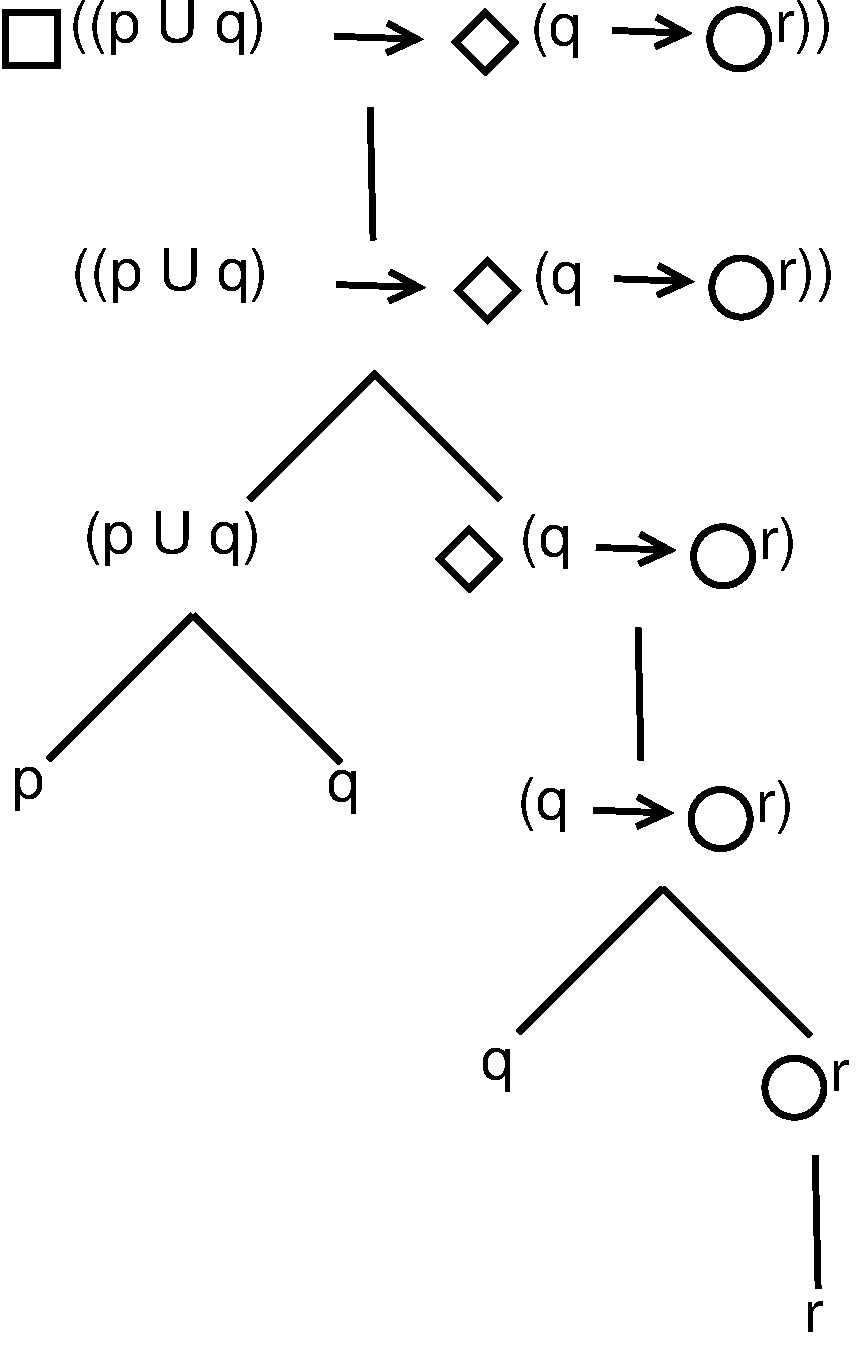
\includegraphics[height=0.3\textheight]{graphics/SubformulaTree}
\label{fig:subformulaTree}
\end{figure}
\\
\qed
\end{myEx}

\begin{description}
\item[Step 2] Walk the tree in breadth-first order to produce a list of subformulae.
\end{description}

\begin{myEx} When we walk the tree in previous example, we get the following subformulae:
\begin{flushleft}
$ \varphi_{1} = \LTLalways((p \,U q) \rightarrow \LTLeventually(q \rightarrow \LTLnext r)) $ \\
$ \varphi_{2} = ((p \,U q) \rightarrow \LTLeventually(q \rightarrow \LTLnext r)) $ \\
$ \varphi_{3} = (p \,U q) $ \\
$ \varphi_{4} = \LTLeventually(q \rightarrow \LTLnext r) $ \\
$ \varphi_{5} = p $ \\
$ \varphi_{6} = q $ \\
$ \varphi_{7} = (q \rightarrow \LTLnext r) $ \\
$ \varphi_{8} = q $ \\
$ \varphi_{9} = \LTLnext r $ \\
$ \varphi_{10} = r $ 
\end{flushleft}
\qed
\end{myEx}

\begin{description}
\item[Step 3] Construct two identical registers called \textit{now} and \textit{next}.  Each register is a one-dimensional array of booleans, where each element corresponds to a formula from the subformulae list, and the length of the array is equal to the length of that list.  Both registers are a permanent breadth-first ordering of the subformula tree.  The first element in the register corresponds to the root of the tree and the last element in the register corresponds to the deepest leaf node of the tree.  The boolean value in each element of the array will hold the truth value that results from evaluating a trace event.\\
\end{description}

\begin{myEx} The now and next registers:\\
\begin{tabular}{cc|c|c|c|c|c|c|c|c|c|c|} &
\multicolumn{1}{c}{} &
\multicolumn{1}{c} {$ \varphi_{1}$} &
\multicolumn{1}{c} {$ \varphi_{2}$} &
\multicolumn{1}{c} {$ \varphi_{3}$} &
\multicolumn{1}{c} {$ \varphi_{4}$} &
\multicolumn{1}{c} {$ \varphi_{5}$} &
\multicolumn{1}{c} {$ \varphi_{6}$} &
\multicolumn{1}{c} {$ \varphi_{7}$} &
\multicolumn{1}{c} {$ \varphi_{8}$} & 
\multicolumn{1}{c} {$ \varphi_{9}$} & 
\multicolumn{1}{c} {$ \varphi_{10}$} \\
\cline{3-12}
& now & $\LTLalways$ & $\rightarrow$ & $U$ & $\LTLeventually$ & $p$ & $q$ & $\rightarrow$ & $q$ & $\LTLnext$ & $r$ \\
\cline{3-12}
\end{tabular}\\
\begin{tabular}{cc|c|c|c|c|c|c|c|c|c|c|} &
\multicolumn{1}{c}{} &
\multicolumn{1}{c} {$ \varphi_{1}$} &
\multicolumn{1}{c} {$ \varphi_{2}$} &
\multicolumn{1}{c} {$ \varphi_{3}$} &
\multicolumn{1}{c} {$ \varphi_{4}$} &
\multicolumn{1}{c} {$ \varphi_{5}$} &
\multicolumn{1}{c} {$ \varphi_{6}$} &
\multicolumn{1}{c} {$ \varphi_{7}$} &
\multicolumn{1}{c} {$ \varphi_{8}$} & 
\multicolumn{1}{c} {$ \varphi_{9}$} & 
\multicolumn{1}{c} {$ \varphi_{10}$} \\
\cline{3-12}
& next & $\LTLalways$ & $\rightarrow$ & $U$ & $\LTLeventually$ & $p$ & $q$ & $\rightarrow$ & $q$ & $\LTLnext$ & $r$ \\
\cline{3-12}
\end{tabular}\\
\qed
\end{myEx}

\begin{description}
\item[Step 4] Before the evaluation phase is performed, the truth values of the \textit{next} register must be initialised.  Traverse the register from the last element to the first, the initial truth value of the element is the value arrived at when evaluating the subformula over an empty trace ($ \epsilon $).  The semantics are those of the future LTL operators and are given in definition \ref{def:FutureEmptyTraceSemantics}.\\
\end{description}

\begin{myEx} Given the example formula $ \varphi = \LTLalways((p \,U q) \rightarrow \LTLeventually(q \rightarrow \LTLnext r))$ the first element to be initialised is the element corresponding to $ \varphi_{10}$, which is the literal r in the subformula tree.  According to semantic rule 1 defined in \ref{def:FutureEmptyTraceSemantics}, a literal over the empty trace evaluates to $ \bot $.  Therefore, after the first element is evaluated the \textit{next} register looks as follows:

\begin{tabular}{cc|c|c|c|c|c|c|c|c|c|c|} &
\multicolumn{1}{c}{} &
\multicolumn{1}{c} {$ \varphi_{1}$} &
\multicolumn{1}{c} {$ \varphi_{2}$} &
\multicolumn{1}{c} {$ \varphi_{3}$} &
\multicolumn{1}{c} {$ \varphi_{4}$} &
\multicolumn{1}{c} {$ \varphi_{5}$} &
\multicolumn{1}{c} {$ \varphi_{6}$} &
\multicolumn{1}{c} {$ \varphi_{7}$} &
\multicolumn{1}{c} {$ \varphi_{8}$} & 
\multicolumn{1}{c} {$ \varphi_{9}$} & 
\multicolumn{1}{c} {$ \varphi_{10}$} \\
\cline{3-12}
& next & $\LTLalways$ & $\rightarrow$ & $U$ & $\LTLeventually$ & $p$ & $q$ & $\rightarrow$ & $q$ & $\LTLnext$ & $\bot$ \\
\cline{3-12}
\end{tabular}\\
\\
\\
The second element to be initialised is $\varphi_{9}$, the formula $\LTLnext r$.  Rule 6 says the next operator evaluates to $ \bot $ over the empty trace:

\begin{tabular}{cc|c|c|c|c|c|c|c|c|c|c|} &
\multicolumn{1}{c}{} &
\multicolumn{1}{c} {$ \varphi_{1}$} &
\multicolumn{1}{c} {$ \varphi_{2}$} &
\multicolumn{1}{c} {$ \varphi_{3}$} &
\multicolumn{1}{c} {$ \varphi_{4}$} &
\multicolumn{1}{c} {$ \varphi_{5}$} &
\multicolumn{1}{c} {$ \varphi_{6}$} &
\multicolumn{1}{c} {$ \varphi_{7}$} &
\multicolumn{1}{c} {$ \varphi_{8}$} & 
\multicolumn{1}{c} {$ \varphi_{9}$} & 
\multicolumn{1}{c} {$ \varphi_{10}$} \\
\cline{3-12}
& next & $\LTLalways$ & $\rightarrow$ & $U$ & $\LTLeventually$ & $p$ & $q$ & $\rightarrow$ & $q$ & $\bot$ & $\bot$ \\
\cline{3-12}
\end{tabular}\\
\\
\\
The next element to be initialised is $\varphi_8$, another literal, therefore it takes the value $\bot$:

\begin{tabular}{cc|c|c|c|c|c|c|c|c|c|c|} &
\multicolumn{1}{c}{} &
\multicolumn{1}{c} {$ \varphi_{1}$} &
\multicolumn{1}{c} {$ \varphi_{2}$} &
\multicolumn{1}{c} {$ \varphi_{3}$} &
\multicolumn{1}{c} {$ \varphi_{4}$} &
\multicolumn{1}{c} {$ \varphi_{5}$} &
\multicolumn{1}{c} {$ \varphi_{6}$} &
\multicolumn{1}{c} {$ \varphi_{7}$} &
\multicolumn{1}{c} {$ \varphi_{8}$} & 
\multicolumn{1}{c} {$ \varphi_{9}$} & 
\multicolumn{1}{c} {$ \varphi_{10}$} \\
\cline{3-12}
& next & $\LTLalways$ & $\rightarrow$ & $U$ & $\LTLeventually$ & $p$ & $q$ & $\rightarrow$ & $\bot$ & $\bot$ & $\bot$ \\
\cline{3-12}
\end{tabular}\\
\\
\\
The formula corresponding to element $\varphi_7$ is $(q \rightarrow \LTLnext r)$.  The semantics of the implies operator are defined by rule 5: The element takes the value of $\top$ when the antecedent is $\bot$.  In this case the antecedent is the literal q and the corresponding element, $\varphi_8$, evaluated to $\bot$ in the previous step.  Therefore $\varphi_7$ takes the value $\top$ because the antecedent evaluates to $ \bot $.  The \textit{next} register is updated to look like:

\begin{tabular}{cc|c|c|c|c|c|c|c|c|c|c|} &
\multicolumn{1}{c}{} &
\multicolumn{1}{c} {$ \varphi_{1}$} &
\multicolumn{1}{c} {$ \varphi_{2}$} &
\multicolumn{1}{c} {$ \varphi_{3}$} &
\multicolumn{1}{c} {$ \varphi_{4}$} &
\multicolumn{1}{c} {$ \varphi_{5}$} &
\multicolumn{1}{c} {$ \varphi_{6}$} &
\multicolumn{1}{c} {$ \varphi_{7}$} &
\multicolumn{1}{c} {$ \varphi_{8}$} & 
\multicolumn{1}{c} {$ \varphi_{9}$} & 
\multicolumn{1}{c} {$ \varphi_{10}$} \\
\cline{3-12}
& next & $\LTLalways$ & $\rightarrow$ & $U$ & $\LTLeventually$ & $p$ & $q$ & $\top$ & $\bot$ & $\bot$ & $\bot$ \\
\cline{3-12}
\end{tabular}\\
\\
\\
This process continues until all the elements of the \textit{next} register have been initialised by evaluation over the empty trace.  The elements in the \textit{now} register are written to by the second phase of the algorithm before they are read, therefore they do not require any initialisation.\\
\\
When the process is complete the two registers appear as follows:\\
\noindent
\begin{tabular}{cc|c|c|c|c|c|c|c|c|c|c|} &
\multicolumn{1}{c}{} &
\multicolumn{1}{c} {$ \varphi_{1}$} &
\multicolumn{1}{c} {$ \varphi_{2}$} &
\multicolumn{1}{c} {$ \varphi_{3}$} &
\multicolumn{1}{c} {$ \varphi_{4}$} &
\multicolumn{1}{c} {$ \varphi_{5}$} &
\multicolumn{1}{c} {$ \varphi_{6}$} &
\multicolumn{1}{c} {$ \varphi_{7}$} &
\multicolumn{1}{c} {$ \varphi_{8}$} & 
\multicolumn{1}{c} {$ \varphi_{9}$} & 
\multicolumn{1}{c} {$ \varphi_{10}$} \\
\cline{3-12}
& next & $\top$ & $\top$ & $\bot$ & $\top$ & $\bot$ & $\bot$ & $\top$ & $\bot$ & $\bot$ & $\bot$\\
\cline{3-12}
\end{tabular}\\
\\
\begin{tabular}{cc|c|c|c|c|c|c|c|c|c|c|} &
\multicolumn{1}{c}{} &
\multicolumn{1}{c} {$ \varphi_{1}$} &
\multicolumn{1}{c} {$ \varphi_{2}$} &
\multicolumn{1}{c} {$ \varphi_{3}$} &
\multicolumn{1}{c} {$ \varphi_{4}$} &
\multicolumn{1}{c} {$ \varphi_{5}$} &
\multicolumn{1}{c} {$ \varphi_{6}$} &
\multicolumn{1}{c} {$ \varphi_{7}$} &
\multicolumn{1}{c} {$ \varphi_{8}$} & 
\multicolumn{1}{c} {$ \varphi_{9}$} & 
\multicolumn{1}{c} {$ \varphi_{10}$} \\
\cline{3-12}
& now & $\LTLalways$ & $\rightarrow$ & $U$ & $\LTLeventually$ & $p$ & $q$ & $\rightarrow$ & $q$ & $\LTLnext$ & $r$ \\
\cline{3-12}
\end{tabular}\\
\\
\qed
\end{myEx}
\noindent That concludes the first phase of the algorithm that produces two registers from an LTL formula.\\  

\section{Evaluation Phase}
\label{sec:EvaluationPhase}
The second phase of the algorithm evaluates the formula over a non-empty trace and is performed for every event in the trace.\\
\begin{description}
%\item[Step 1] When a new event occurs add that event to the end of the trace.

\item[Step 1] Traverse the trace from the last entry to the first, taking each entry from the trace.  With that entry iterate over the \textit{now} register from last element to the first, evaluating the corresponding subformula over the trace entry, according to the operator's semantics from definition \ref{def:FutureNon-emptyTraceSemantics}.  Assign the resulting truth value to the element.

\item[Step 2] next[i] = now[i] for all i ranging from 1..length(now).

\item[Step 3] Repeat steps 1 and 2 with the preceding (earlier) trace entry until arriving at the head of the trace where there is no preceding entry.

\item[Step 4] The final result of evaluating the formula over the trace is found as the truth value of the first element in the \textit{next} register because this element corresponds to the root of the subformula tree.\\
\end{description}

Understanding steps 1 and 2 is key to understanding the \RH\ algorithm and how it evaluates the temporal operators of LTL.  There are three elements to understanding these steps, the \textit{next} register, the relation between the \textit{now} register and the \textit{next} register and the order that the trace is evaluated.

To explain how to evaluate a trace event in relation to the registers, we have to adapt the semantics from definition \ref{def:FutureNon-emptyTraceSemantics} to refer to the registers.  We replace $e$ with a reference to the \textit{now} register and $t$ becomes the \textit{next} register.  The subformulae of $ \varphi $ are replaced with references to the corresponding elements within the \textit{now} and \textit{next} registers by the use of indices $i$, $j$, and $k$.  The index $i$ maps to the element corresponding to the subformula's operator.  Indices $j$ and $k$ map to the elements corresponding to the left and right operands respectively.  The registers are a permanent breadth-first ordering of the subformula tree, so an operator comes before it's operands in a register, thus $i < j < k$.\\
\newpage
\begin{definition}Algorithmic Operator Semantics\\
\label{def:AlgorithmicOperatorSemantics}
\\
For a given trace event $e$, for all $i$ ranging from length(\textit{now})..1, if the $i^{th}$ outermost operator is:
\begin{enumerate}
\item literal l, then \textit{now}[$i$] $ \leftarrow $ (l == $e$)
\item $ \neg $ then \textit{now}[$i$] $ \leftarrow $ NOT(\textit{now}[$j$]).
\item $ \lor $ then \textit{now}[$i$] $ \leftarrow $ \textit{now}[$j$] OR \textit{now}[$k$]. 
\item $ \land $ then \textit{now}[$i$] $ \leftarrow $ \textit{now}[$j$] AND \textit{now}[$k$]. 
\item $ \rightarrow $ then now[$i$] $ \leftarrow $ NOT(\textit{now}[$j$]) OR \textit{now}[$k$]. 
\item $ \LTLnext $ then \textit{now}[$i$] $ \leftarrow $ \textit{next}[$j$].
\item $ \LTLalways $ then \textit{now}[$i$] $ \leftarrow $ \textit{now}[$j$] AND \textit{next}[$i$].
\item $ \LTLeventually $ then \textit{now}[$i$] $ \leftarrow $ \textit{now}[$j$] OR \textit{next}[$i$].
\item U then \textit{now}[$i$] $ \leftarrow $ \textit{now}[$k$] OR (\textit{now}[$j$] AND \textit{next}[$i$]).
\end{enumerate}
\end{definition}

The reader may notice that the boolean operators $ \neg, \lor, \land, \rightarrow $ only reference other elements in the \textit{now} register.  This is because the semantics of these operators do not depend on any other events within the trace.  Whereas the semantics of the temporal operators $ \LTLnext, \ \LTLalways,  \ \LTLeventually, \ U $ depend on events that may have occurred elsewhere in the trace so they also reference the \textit{next} register.

The \textit{next} register represents the cumulative evaluations of all trace events after the event currently being evaluated.  Following each evaluation of an event, the elements of the \textit{next} register get set to the corresponding values from the \textit{now} register.  But we can see that evaluation of the \textit{now} register is itself based upon the earlier state of the \textit{next} register.  This circular-referencing process accumulates all prior evaluations into the \textit{next} register.  Because the trace gets evaluated from the latest entry to the earliest, those prior evaluations are all the events that occurred after the current event.  Therefore the evaluation of each event in the trace is based upon the prior evaluation of events that come after.

Evaluating events from latest to earliest explains why the algorithm is limited to implementing only the future LTL operators; when evaluating an event only the evaluations of `future' events are known.
\newpage
\begin{myEx}
Example evaluation of a trace $t$ that satisfies $\varphi$\\
\\
$t = \langle p, q, r \rangle$\\
$\varphi = \LTLalways((p \,U q) \rightarrow \LTLeventually(q \rightarrow \LTLnext r))$

\textbf{\item[Phase 1]- Initialisation}\\

The two registers are initialised and the result is the same as in Example 9:\\
\begin{tabular}{cc|c|c|c|c|c|c|c|c|c|c|} &
\multicolumn{1}{c}{} &
\multicolumn{1}{c} {$ \varphi_{1}$} &
\multicolumn{1}{c} {$ \varphi_{2}$} &
\multicolumn{1}{c} {$ \varphi_{3}$} &
\multicolumn{1}{c} {$ \varphi_{4}$} &
\multicolumn{1}{c} {$ \varphi_{5}$} &
\multicolumn{1}{c} {$ \varphi_{6}$} &
\multicolumn{1}{c} {$ \varphi_{7}$} &
\multicolumn{1}{c} {$ \varphi_{8}$} & 
\multicolumn{1}{c} {$ \varphi_{9}$} & 
\multicolumn{1}{c} {$ \varphi_{10}$} \\
\cline{3-12}
& next & $ \top $ & $ \top $ & $ \bot $ & $ \top $ & $ \bot $ & $ \bot $ & $ \top $ & $ \bot $ & $ \bot $ & $ \bot $ \\
\cline{3-12}
\end{tabular}\\
\\
\begin{tabular}{cc|c|c|c|c|c|c|c|c|c|c|} &
\multicolumn{1}{c}{} &
\multicolumn{1}{c} {$ \varphi_{1}$} &
\multicolumn{1}{c} {$ \varphi_{2}$} &
\multicolumn{1}{c} {$ \varphi_{3}$} &
\multicolumn{1}{c} {$ \varphi_{4}$} &
\multicolumn{1}{c} {$ \varphi_{5}$} &
\multicolumn{1}{c} {$ \varphi_{6}$} &
\multicolumn{1}{c} {$ \varphi_{7}$} &
\multicolumn{1}{c} {$ \varphi_{8}$} & 
\multicolumn{1}{c} {$ \varphi_{9}$} & 
\multicolumn{1}{c} {$ \varphi_{10}$} \\
\cline{3-12}
& now & $\LTLalways$ & $\rightarrow$ & $U$ & $\LTLeventually$ & $p$ & $q$ & $\rightarrow$ & $q$ & $\LTLnext$ & $r$ \\
\cline{3-12}
\end{tabular}\\

\textbf{\item[Phase 2]- Evaluation}\\

The evaluation phase determines if the trace satisfies the formula.  The formula is said to be satisfied if the formula evaluates to $\top$ after considering every event in the trace, from the last event to the earliest.  When considering each event, the algorithm iterates over every element in the \textit{now} register from the last element downto the first, and evaluates the event over the subformula corresponding to that element.  At each iteration the index $i$ references the element being evaluated and indices $j$ and $k$ reference the elements that correspond to the left and right operands of the subformula.

% =====
% Event 1
% =====
\textbf{\item Evaluation Phase - Step 1}\\

\subitem \underline{Event 1, Iteration 1: $t = \langle p, q, r \rangle, e = r, i = 10$}\\
\\
Registers before:\\

\begin{tabular}{cc|c|c|c|c|c|c|c|c|c|c|} &
\multicolumn{1}{c}{} &
\multicolumn{1}{c} {$ \varphi_{1}$} &
\multicolumn{1}{c} {$ \varphi_{2}$} &
\multicolumn{1}{c} {$ \varphi_{3}$} &
\multicolumn{1}{c} {$ \varphi_{4}$} &
\multicolumn{1}{c} {$ \varphi_{5}$} &
\multicolumn{1}{c} {$ \varphi_{6}$} &
\multicolumn{1}{c} {$ \varphi_{7}$} &
\multicolumn{1}{c} {$ \varphi_{8}$} & 
\multicolumn{1}{c} {$ \varphi_{9}$} & 
\multicolumn{1}{c} {$ \varphi_{10}$} \\
\cline{3-12}
& next & $ \top $ & $ \top $ & $ \bot $ & $ \top $ & $ \bot $ & $ \bot $ & $ \top $ & $ \bot $ & $ \bot $ & $ \bot $ \\
\cline{3-12}
\end{tabular}\\

\begin{tabular}{cc|c|c|c|c|c|c|c|c|c|c|} &
\multicolumn{1}{c}{} &
\multicolumn{1}{c} {$ \varphi_{1}$} &
\multicolumn{1}{c} {$ \varphi_{2}$} &
\multicolumn{1}{c} {$ \varphi_{3}$} &
\multicolumn{1}{c} {$ \varphi_{4}$} &
\multicolumn{1}{c} {$ \varphi_{5}$} &
\multicolumn{1}{c} {$ \varphi_{6}$} &
\multicolumn{1}{c} {$ \varphi_{7}$} &
\multicolumn{1}{c} {$ \varphi_{8}$} & 
\multicolumn{1}{c} {$ \varphi_{9}$} & 
\multicolumn{1}{c} {$ \varphi_{10}$} \\
\cline{3-12}
& now & $\LTLalways$ & $\rightarrow$ & $U$ & $\LTLeventually$ & $p$ & $q$ & $\rightarrow$ & $q$ & $\LTLnext$ & $r$ \\
\cline{3-12}
\end{tabular}\\
\\
\\
The first event being considered is the last event in the trace, the event $r$.  Given that event, the algorithm iterates over each element in the \textit{now} register, from element $10$ downto $1$.  The index $i$ = 10, so the first element to be evaluated is $now[10]$ that corresponds to subformulae $\varphi_{10}$, the literal $r$.  The event being considered is $r$, therefore by rule 1 of Definition \ref{def:AlgorithmicOperatorSemantics}, the element evaluates to $\top$.\\

\newpage

Registers after:\\

\begin{tabular}{cc|c|c|c|c|c|c|c|c|c|c|} &
\multicolumn{1}{c}{} &
\multicolumn{1}{c} {$ \varphi_{1}$} &
\multicolumn{1}{c} {$ \varphi_{2}$} &
\multicolumn{1}{c} {$ \varphi_{3}$} &
\multicolumn{1}{c} {$ \varphi_{4}$} &
\multicolumn{1}{c} {$ \varphi_{5}$} &
\multicolumn{1}{c} {$ \varphi_{6}$} &
\multicolumn{1}{c} {$ \varphi_{7}$} &
\multicolumn{1}{c} {$ \varphi_{8}$} & 
\multicolumn{1}{c} {$ \varphi_{9}$} & 
\multicolumn{1}{c} {$ \varphi_{10}$} \\
\cline{3-12}
& next & $ \top $ & $ \top $ & $ \bot $ & $ \top $ & $ \bot $ & $ \bot $ & $ \top $ & $ \bot $ & $ \bot $ & $ \bot $ \\
\cline{3-12}
\end{tabular}\\

\begin{tabular}{cc|c|c|c|c|c|c|c|c|c|c|} &
\multicolumn{1}{c}{} &
\multicolumn{1}{c} {$ \varphi_{1}$} &
\multicolumn{1}{c} {$ \varphi_{2}$} &
\multicolumn{1}{c} {$ \varphi_{3}$} &
\multicolumn{1}{c} {$ \varphi_{4}$} &
\multicolumn{1}{c} {$ \varphi_{5}$} &
\multicolumn{1}{c} {$ \varphi_{6}$} &
\multicolumn{1}{c} {$ \varphi_{7}$} &
\multicolumn{1}{c} {$ \varphi_{8}$} & 
\multicolumn{1}{c} {$ \varphi_{9}$} & 
\multicolumn{1}{c} {$ \varphi_{10}$} \\
\cline{3-12}
& now & $\LTLalways$ & $\rightarrow$ & $U$ & $\LTLeventually$ & $p$ & $q$ & $\rightarrow$ & $q$ & $\LTLnext$ & $\top$ \\
\cline{3-12}
\end{tabular}\\
\\
\\
\subitem \underline{Event 1, Iteration 2: $t = \langle p, q, r \rangle, e = r, i = 9, j = 10$}\\
\\
Registers before:\\

\begin{tabular}{cc|c|c|c|c|c|c|c|c|c|c|} &
\multicolumn{1}{c}{} &
\multicolumn{1}{c} {$ \varphi_{1}$} &
\multicolumn{1}{c} {$ \varphi_{2}$} &
\multicolumn{1}{c} {$ \varphi_{3}$} &
\multicolumn{1}{c} {$ \varphi_{4}$} &
\multicolumn{1}{c} {$ \varphi_{5}$} &
\multicolumn{1}{c} {$ \varphi_{6}$} &
\multicolumn{1}{c} {$ \varphi_{7}$} &
\multicolumn{1}{c} {$ \varphi_{8}$} & 
\multicolumn{1}{c} {$ \varphi_{9}$} & 
\multicolumn{1}{c} {$ \varphi_{10}$} \\
\cline{3-12}
& next & $ \top $ & $ \top $ & $ \bot $ & $ \top $ & $ \bot $ & $ \bot $ & $ \top $ & $ \bot $ & $ \bot $ & $ \bot $ \\
\cline{3-12}
\end{tabular}\\

\begin{tabular}{cc|c|c|c|c|c|c|c|c|c|c|} &
\multicolumn{1}{c}{} &
\multicolumn{1}{c} {$ \varphi_{1}$} &
\multicolumn{1}{c} {$ \varphi_{2}$} &
\multicolumn{1}{c} {$ \varphi_{3}$} &
\multicolumn{1}{c} {$ \varphi_{4}$} &
\multicolumn{1}{c} {$ \varphi_{5}$} &
\multicolumn{1}{c} {$ \varphi_{6}$} &
\multicolumn{1}{c} {$ \varphi_{7}$} &
\multicolumn{1}{c} {$ \varphi_{8}$} & 
\multicolumn{1}{c} {$ \varphi_{9}$} & 
\multicolumn{1}{c} {$ \varphi_{10}$} \\
\cline{3-12}
& now & $\LTLalways$ & $\rightarrow$ & $U$ & $\LTLeventually$ & $p$ & $q$ & $\rightarrow$ & $q$ & $\LTLnext$ & $\top$ \\
\cline{3-12}
\end{tabular}\\
\\
\\
The second iteration evaluates the element corresponding to subformula $\varphi_{9}$, $\LTLnext r$.  The outermost operator of the subformula is the next operator, thus rule 6 applies.  The semantics are that the subformula evaluates $\top$ if the following event in the trace satisfies the left operand.  The \textit{next} register tells us how events that come later in the trace were evaluated, and the left operand of a subformula is referenced by the index $j$.  Therefore by rule 6, $now[9]$ is assigned the value from $next[10]$, which is $\bot$.\\
\\
Registers after:\\

\begin{tabular}{cc|c|c|c|c|c|c|c|c|c|c|} &
\multicolumn{1}{c}{} &
\multicolumn{1}{c} {$ \varphi_{1}$} &
\multicolumn{1}{c} {$ \varphi_{2}$} &
\multicolumn{1}{c} {$ \varphi_{3}$} &
\multicolumn{1}{c} {$ \varphi_{4}$} &
\multicolumn{1}{c} {$ \varphi_{5}$} &
\multicolumn{1}{c} {$ \varphi_{6}$} &
\multicolumn{1}{c} {$ \varphi_{7}$} &
\multicolumn{1}{c} {$ \varphi_{8}$} & 
\multicolumn{1}{c} {$ \varphi_{9}$} & 
\multicolumn{1}{c} {$ \varphi_{10}$} \\
\cline{3-12}
& next & $ \top $ & $ \top $ & $ \bot $ & $ \top $ & $ \bot $ & $ \bot $ & $ \top $ & $ \bot $ & $ \bot $ & $ \bot $ \\
\cline{3-12}
\end{tabular}\\

\begin{tabular}{cc|c|c|c|c|c|c|c|c|c|c|} &
\multicolumn{1}{c}{} &
\multicolumn{1}{c} {$ \varphi_{1}$} &
\multicolumn{1}{c} {$ \varphi_{2}$} &
\multicolumn{1}{c} {$ \varphi_{3}$} &
\multicolumn{1}{c} {$ \varphi_{4}$} &
\multicolumn{1}{c} {$ \varphi_{5}$} &
\multicolumn{1}{c} {$ \varphi_{6}$} &
\multicolumn{1}{c} {$ \varphi_{7}$} &
\multicolumn{1}{c} {$ \varphi_{8}$} & 
\multicolumn{1}{c} {$ \varphi_{9}$} & 
\multicolumn{1}{c} {$ \varphi_{10}$} \\
\cline{3-12}
& now & $\LTLalways$ & $\rightarrow$ & $U$ & $\LTLeventually$ & $p$ & $q$ & $\rightarrow$ & $q$ & $\bot$ & $\top$ \\
\cline{3-12}
\end{tabular}\\
\\
\\
\newpage
\subitem \underline{Event 1, Iteration 3: $t = \langle p, q, r \rangle, e = r, i = 8$}\\
\\
Registers before:\\

\begin{tabular}{cc|c|c|c|c|c|c|c|c|c|c|} &
\multicolumn{1}{c}{} &
\multicolumn{1}{c} {$ \varphi_{1}$} &
\multicolumn{1}{c} {$ \varphi_{2}$} &
\multicolumn{1}{c} {$ \varphi_{3}$} &
\multicolumn{1}{c} {$ \varphi_{4}$} &
\multicolumn{1}{c} {$ \varphi_{5}$} &
\multicolumn{1}{c} {$ \varphi_{6}$} &
\multicolumn{1}{c} {$ \varphi_{7}$} &
\multicolumn{1}{c} {$ \varphi_{8}$} & 
\multicolumn{1}{c} {$ \varphi_{9}$} & 
\multicolumn{1}{c} {$ \varphi_{10}$} \\
\cline{3-12}
& next & $ \top $ & $ \top $ & $ \bot $ & $ \top $ & $ \bot $ & $ \bot $ & $ \top $ & $ \bot $ & $ \bot $ & $ \bot $ \\
\cline{3-12}
\end{tabular}\\

\begin{tabular}{cc|c|c|c|c|c|c|c|c|c|c|} &
\multicolumn{1}{c}{} &
\multicolumn{1}{c} {$ \varphi_{1}$} &
\multicolumn{1}{c} {$ \varphi_{2}$} &
\multicolumn{1}{c} {$ \varphi_{3}$} &
\multicolumn{1}{c} {$ \varphi_{4}$} &
\multicolumn{1}{c} {$ \varphi_{5}$} &
\multicolumn{1}{c} {$ \varphi_{6}$} &
\multicolumn{1}{c} {$ \varphi_{7}$} &
\multicolumn{1}{c} {$ \varphi_{8}$} & 
\multicolumn{1}{c} {$ \varphi_{9}$} & 
\multicolumn{1}{c} {$ \varphi_{10}$} \\
\cline{3-12}
& now & $\LTLalways$ & $\rightarrow$ & $U$ & $\LTLeventually$ & $p$ & $q$ & $\rightarrow$ & $q$ & $\bot$ & $\top$ \\
\cline{3-12}
\end{tabular}\\
\\
\\
Cell $now[8]$ corresponds to the literal $q$.  The event being considered is $r$, therefore by rule 1, $now[8]$ evaluates to $\bot$.\\
\\
Registers after:\\

\begin{tabular}{cc|c|c|c|c|c|c|c|c|c|c|} &
\multicolumn{1}{c}{} &
\multicolumn{1}{c} {$ \varphi_{1}$} &
\multicolumn{1}{c} {$ \varphi_{2}$} &
\multicolumn{1}{c} {$ \varphi_{3}$} &
\multicolumn{1}{c} {$ \varphi_{4}$} &
\multicolumn{1}{c} {$ \varphi_{5}$} &
\multicolumn{1}{c} {$ \varphi_{6}$} &
\multicolumn{1}{c} {$ \varphi_{7}$} &
\multicolumn{1}{c} {$ \varphi_{8}$} & 
\multicolumn{1}{c} {$ \varphi_{9}$} & 
\multicolumn{1}{c} {$ \varphi_{10}$} \\
\cline{3-12}
& next & $ \top $ & $ \top $ & $ \bot $ & $ \top $ & $ \bot $ & $ \bot $ & $ \top $ & $ \bot $ & $ \bot $ & $ \bot $ \\
\cline{3-12}
\end{tabular}\\

\begin{tabular}{cc|c|c|c|c|c|c|c|c|c|c|} &
\multicolumn{1}{c}{} &
\multicolumn{1}{c} {$ \varphi_{1}$} &
\multicolumn{1}{c} {$ \varphi_{2}$} &
\multicolumn{1}{c} {$ \varphi_{3}$} &
\multicolumn{1}{c} {$ \varphi_{4}$} &
\multicolumn{1}{c} {$ \varphi_{5}$} &
\multicolumn{1}{c} {$ \varphi_{6}$} &
\multicolumn{1}{c} {$ \varphi_{7}$} &
\multicolumn{1}{c} {$ \varphi_{8}$} & 
\multicolumn{1}{c} {$ \varphi_{9}$} & 
\multicolumn{1}{c} {$ \varphi_{10}$} \\
\cline{3-12}
& now & $\LTLalways$ & $\rightarrow$ & $U$ & $\LTLeventually$ & $p$ & $q$ & $\rightarrow$ & $\bot$ & $\bot$ & $\top$ \\
\cline{3-12}
\end{tabular}\\
\\
\\
\subitem \underline{Event 1, Iteration 4: $t = \langle p, q, r \rangle, e = r, i = 7, j = 8, k = 9$}\\
\\
Registers before:\\

\begin{tabular}{cc|c|c|c|c|c|c|c|c|c|c|} &
\multicolumn{1}{c}{} &
\multicolumn{1}{c} {$ \varphi_{1}$} &
\multicolumn{1}{c} {$ \varphi_{2}$} &
\multicolumn{1}{c} {$ \varphi_{3}$} &
\multicolumn{1}{c} {$ \varphi_{4}$} &
\multicolumn{1}{c} {$ \varphi_{5}$} &
\multicolumn{1}{c} {$ \varphi_{6}$} &
\multicolumn{1}{c} {$ \varphi_{7}$} &
\multicolumn{1}{c} {$ \varphi_{8}$} & 
\multicolumn{1}{c} {$ \varphi_{9}$} & 
\multicolumn{1}{c} {$ \varphi_{10}$} \\
\cline{3-12}
& next & $ \top $ & $ \top $ & $ \bot $ & $ \top $ & $ \bot $ & $ \bot $ & $ \top $ & $ \bot $ & $ \bot $ & $ \bot $ \\
\cline{3-12}
\end{tabular}\\

\begin{tabular}{cc|c|c|c|c|c|c|c|c|c|c|} &
\multicolumn{1}{c}{} &
\multicolumn{1}{c} {$ \varphi_{1}$} &
\multicolumn{1}{c} {$ \varphi_{2}$} &
\multicolumn{1}{c} {$ \varphi_{3}$} &
\multicolumn{1}{c} {$ \varphi_{4}$} &
\multicolumn{1}{c} {$ \varphi_{5}$} &
\multicolumn{1}{c} {$ \varphi_{6}$} &
\multicolumn{1}{c} {$ \varphi_{7}$} &
\multicolumn{1}{c} {$ \varphi_{8}$} & 
\multicolumn{1}{c} {$ \varphi_{9}$} & 
\multicolumn{1}{c} {$ \varphi_{10}$} \\
\cline{3-12}
& now & $\LTLalways$ & $\rightarrow$ & $U$ & $\LTLeventually$ & $p$ & $q$ & $\rightarrow$ & $\bot$ & $\bot$ & $\top$ \\
\cline{3-12}
\end{tabular}\\
\\
\\
Cell $now[7]$ corresponds to the $(q \rightarrow \LTLnext r)$ subformula, with implies as the outermost operator.  Rule 5 defines the implies operator and assigns $\top$ to $now[7]$ if the left operand is $\bot$ or the right operand is $\top$.  In this case the left operand is referenced by the $j$ index and is element $now[8]$.  It has the value $\bot$, therefore $now[7]$ is assigned $\top$.\\
\\
\newpage
Registers after:\\

\begin{tabular}{cc|c|c|c|c|c|c|c|c|c|c|} &
\multicolumn{1}{c}{} &
\multicolumn{1}{c} {$ \varphi_{1}$} &
\multicolumn{1}{c} {$ \varphi_{2}$} &
\multicolumn{1}{c} {$ \varphi_{3}$} &
\multicolumn{1}{c} {$ \varphi_{4}$} &
\multicolumn{1}{c} {$ \varphi_{5}$} &
\multicolumn{1}{c} {$ \varphi_{6}$} &
\multicolumn{1}{c} {$ \varphi_{7}$} &
\multicolumn{1}{c} {$ \varphi_{8}$} & 
\multicolumn{1}{c} {$ \varphi_{9}$} & 
\multicolumn{1}{c} {$ \varphi_{10}$} \\
\cline{3-12}
& next & $ \top $ & $ \top $ & $ \bot $ & $ \top $ & $ \bot $ & $ \bot $ & $ \top $ & $ \bot $ & $ \bot $ & $ \bot $ \\
\cline{3-12}
\end{tabular}\\

\begin{tabular}{cc|c|c|c|c|c|c|c|c|c|c|} &
\multicolumn{1}{c}{} &
\multicolumn{1}{c} {$ \varphi_{1}$} &
\multicolumn{1}{c} {$ \varphi_{2}$} &
\multicolumn{1}{c} {$ \varphi_{3}$} &
\multicolumn{1}{c} {$ \varphi_{4}$} &
\multicolumn{1}{c} {$ \varphi_{5}$} &
\multicolumn{1}{c} {$ \varphi_{6}$} &
\multicolumn{1}{c} {$ \varphi_{7}$} &
\multicolumn{1}{c} {$ \varphi_{8}$} & 
\multicolumn{1}{c} {$ \varphi_{9}$} & 
\multicolumn{1}{c} {$ \varphi_{10}$} \\
\cline{3-12}
& now & $\LTLalways$ & $\rightarrow$ & $U$ & $\LTLeventually$ & $p$ & $q$ & $\top$ & $\bot$ & $\bot$ & $\top$ \\
\cline{3-12}
\end{tabular}\\
\\
\\
\subitem \underline{Event 1, Iteration 5: $t = \langle p, q, r \rangle, e = r, i = 6$}\\
\\
Registers before:\\

\begin{tabular}{cc|c|c|c|c|c|c|c|c|c|c|} &
\multicolumn{1}{c}{} &
\multicolumn{1}{c} {$ \varphi_{1}$} &
\multicolumn{1}{c} {$ \varphi_{2}$} &
\multicolumn{1}{c} {$ \varphi_{3}$} &
\multicolumn{1}{c} {$ \varphi_{4}$} &
\multicolumn{1}{c} {$ \varphi_{5}$} &
\multicolumn{1}{c} {$ \varphi_{6}$} &
\multicolumn{1}{c} {$ \varphi_{7}$} &
\multicolumn{1}{c} {$ \varphi_{8}$} & 
\multicolumn{1}{c} {$ \varphi_{9}$} & 
\multicolumn{1}{c} {$ \varphi_{10}$} \\
\cline{3-12}
& next & $ \top $ & $ \top $ & $ \bot $ & $ \top $ & $ \bot $ & $ \bot $ & $ \top $ & $ \bot $ & $ \bot $ & $ \bot $ \\
\cline{3-12}
\end{tabular}\\

\begin{tabular}{cc|c|c|c|c|c|c|c|c|c|c|} &
\multicolumn{1}{c}{} &
\multicolumn{1}{c} {$ \varphi_{1}$} &
\multicolumn{1}{c} {$ \varphi_{2}$} &
\multicolumn{1}{c} {$ \varphi_{3}$} &
\multicolumn{1}{c} {$ \varphi_{4}$} &
\multicolumn{1}{c} {$ \varphi_{5}$} &
\multicolumn{1}{c} {$ \varphi_{6}$} &
\multicolumn{1}{c} {$ \varphi_{7}$} &
\multicolumn{1}{c} {$ \varphi_{8}$} & 
\multicolumn{1}{c} {$ \varphi_{9}$} & 
\multicolumn{1}{c} {$ \varphi_{10}$} \\
\cline{3-12}
& now & $\LTLalways$ & $\rightarrow$ & $U$ & $\LTLeventually$ & $p$ & $q$ & $\top$ & $\bot$ & $\bot$ & $\top$ \\
\cline{3-12}
\end{tabular}\\
\\
\\
Cell $now[6]$ corresponds to the literal $q$.  The event being considered is $r$, therefore by rule 1, $now[6]$ evaluates to $\bot$.\\
\\
Registers after:\\

\begin{tabular}{cc|c|c|c|c|c|c|c|c|c|c|} &
\multicolumn{1}{c}{} &
\multicolumn{1}{c} {$ \varphi_{1}$} &
\multicolumn{1}{c} {$ \varphi_{2}$} &
\multicolumn{1}{c} {$ \varphi_{3}$} &
\multicolumn{1}{c} {$ \varphi_{4}$} &
\multicolumn{1}{c} {$ \varphi_{5}$} &
\multicolumn{1}{c} {$ \varphi_{6}$} &
\multicolumn{1}{c} {$ \varphi_{7}$} &
\multicolumn{1}{c} {$ \varphi_{8}$} & 
\multicolumn{1}{c} {$ \varphi_{9}$} & 
\multicolumn{1}{c} {$ \varphi_{10}$} \\
\cline{3-12}
& next & $ \top $ & $ \top $ & $ \bot $ & $ \top $ & $ \bot $ & $ \bot $ & $ \top $ & $ \bot $ & $ \bot $ & $ \bot $ \\
\cline{3-12}
\end{tabular}\\

\begin{tabular}{cc|c|c|c|c|c|c|c|c|c|c|} &
\multicolumn{1}{c}{} &
\multicolumn{1}{c} {$ \varphi_{1}$} &
\multicolumn{1}{c} {$ \varphi_{2}$} &
\multicolumn{1}{c} {$ \varphi_{3}$} &
\multicolumn{1}{c} {$ \varphi_{4}$} &
\multicolumn{1}{c} {$ \varphi_{5}$} &
\multicolumn{1}{c} {$ \varphi_{6}$} &
\multicolumn{1}{c} {$ \varphi_{7}$} &
\multicolumn{1}{c} {$ \varphi_{8}$} & 
\multicolumn{1}{c} {$ \varphi_{9}$} & 
\multicolumn{1}{c} {$ \varphi_{10}$} \\
\cline{3-12}
& now & $\LTLalways$ & $\rightarrow$ & $U$ & $\LTLeventually$ & $p$ & $\bot$ & $\top$ & $\bot$ & $\bot$ & $\top$ \\
\cline{3-12}
\end{tabular}\\
\\
\\
\subitem \underline{Event 1, Iteration 6: $t = \langle p, q, r \rangle, e = r, i = 5$}\\
\\
Registers before:\\

\begin{tabular}{cc|c|c|c|c|c|c|c|c|c|c|} &
\multicolumn{1}{c}{} &
\multicolumn{1}{c} {$ \varphi_{1}$} &
\multicolumn{1}{c} {$ \varphi_{2}$} &
\multicolumn{1}{c} {$ \varphi_{3}$} &
\multicolumn{1}{c} {$ \varphi_{4}$} &
\multicolumn{1}{c} {$ \varphi_{5}$} &
\multicolumn{1}{c} {$ \varphi_{6}$} &
\multicolumn{1}{c} {$ \varphi_{7}$} &
\multicolumn{1}{c} {$ \varphi_{8}$} & 
\multicolumn{1}{c} {$ \varphi_{9}$} & 
\multicolumn{1}{c} {$ \varphi_{10}$} \\
\cline{3-12}
& next & $ \top $ & $ \top $ & $ \bot $ & $ \top $ & $ \bot $ & $ \bot $ & $ \top $ & $ \bot $ & $ \bot $ & $ \bot $ \\
\cline{3-12}
\end{tabular}\\

\begin{tabular}{cc|c|c|c|c|c|c|c|c|c|c|} &
\multicolumn{1}{c}{} &
\multicolumn{1}{c} {$ \varphi_{1}$} &
\multicolumn{1}{c} {$ \varphi_{2}$} &
\multicolumn{1}{c} {$ \varphi_{3}$} &
\multicolumn{1}{c} {$ \varphi_{4}$} &
\multicolumn{1}{c} {$ \varphi_{5}$} &
\multicolumn{1}{c} {$ \varphi_{6}$} &
\multicolumn{1}{c} {$ \varphi_{7}$} &
\multicolumn{1}{c} {$ \varphi_{8}$} & 
\multicolumn{1}{c} {$ \varphi_{9}$} & 
\multicolumn{1}{c} {$ \varphi_{10}$} \\
\cline{3-12}
& now & $\LTLalways$ & $\rightarrow$ & $U$ & $\LTLeventually$ & $p$ & $\bot$ & $\top$ & $\bot$ & $\bot$ & $\top$ \\
\cline{3-12}
\end{tabular}\\
\\
\\
Cell $now[5]$ corresponds to the literal $p$.  The event being considered is $r$, therefore by rule 1, $now[5]$ evaluates to $\bot$.\\
\\
Registers after:\\

\begin{tabular}{cc|c|c|c|c|c|c|c|c|c|c|} &
\multicolumn{1}{c}{} &
\multicolumn{1}{c} {$ \varphi_{1}$} &
\multicolumn{1}{c} {$ \varphi_{2}$} &
\multicolumn{1}{c} {$ \varphi_{3}$} &
\multicolumn{1}{c} {$ \varphi_{4}$} &
\multicolumn{1}{c} {$ \varphi_{5}$} &
\multicolumn{1}{c} {$ \varphi_{6}$} &
\multicolumn{1}{c} {$ \varphi_{7}$} &
\multicolumn{1}{c} {$ \varphi_{8}$} & 
\multicolumn{1}{c} {$ \varphi_{9}$} & 
\multicolumn{1}{c} {$ \varphi_{10}$} \\
\cline{3-12}
& next & $ \top $ & $ \top $ & $ \bot $ & $ \top $ & $ \bot $ & $ \bot $ & $ \top $ & $ \bot $ & $ \bot $ & $ \bot $ \\
\cline{3-12}
\end{tabular}\\

\begin{tabular}{cc|c|c|c|c|c|c|c|c|c|c|} &
\multicolumn{1}{c}{} &
\multicolumn{1}{c} {$ \varphi_{1}$} &
\multicolumn{1}{c} {$ \varphi_{2}$} &
\multicolumn{1}{c} {$ \varphi_{3}$} &
\multicolumn{1}{c} {$ \varphi_{4}$} &
\multicolumn{1}{c} {$ \varphi_{5}$} &
\multicolumn{1}{c} {$ \varphi_{6}$} &
\multicolumn{1}{c} {$ \varphi_{7}$} &
\multicolumn{1}{c} {$ \varphi_{8}$} & 
\multicolumn{1}{c} {$ \varphi_{9}$} & 
\multicolumn{1}{c} {$ \varphi_{10}$} \\
\cline{3-12}
& now & $\LTLalways$ & $\rightarrow$ & $U$ & $\LTLeventually$ & $\bot$ & $\bot$ & $\top$ & $\bot$ & $\bot$ & $\top$ \\
\cline{3-12}
\end{tabular}\\
\\
\\
\subitem \underline{Event 1, Iteration 7: $t = \langle p, q, r \rangle, e = r, i = 4, j = 7$}\\
\\
Registers before:\\

\begin{tabular}{cc|c|c|c|c|c|c|c|c|c|c|} &
\multicolumn{1}{c}{} &
\multicolumn{1}{c} {$ \varphi_{1}$} &
\multicolumn{1}{c} {$ \varphi_{2}$} &
\multicolumn{1}{c} {$ \varphi_{3}$} &
\multicolumn{1}{c} {$ \varphi_{4}$} &
\multicolumn{1}{c} {$ \varphi_{5}$} &
\multicolumn{1}{c} {$ \varphi_{6}$} &
\multicolumn{1}{c} {$ \varphi_{7}$} &
\multicolumn{1}{c} {$ \varphi_{8}$} & 
\multicolumn{1}{c} {$ \varphi_{9}$} & 
\multicolumn{1}{c} {$ \varphi_{10}$} \\
\cline{3-12}
& next & $ \top $ & $ \top $ & $ \bot $ & $ \top $ & $ \bot $ & $ \bot $ & $ \top $ & $ \bot $ & $ \bot $ & $ \bot $ \\
\cline{3-12}
\end{tabular}\\

\begin{tabular}{cc|c|c|c|c|c|c|c|c|c|c|} &
\multicolumn{1}{c}{} &
\multicolumn{1}{c} {$ \varphi_{1}$} &
\multicolumn{1}{c} {$ \varphi_{2}$} &
\multicolumn{1}{c} {$ \varphi_{3}$} &
\multicolumn{1}{c} {$ \varphi_{4}$} &
\multicolumn{1}{c} {$ \varphi_{5}$} &
\multicolumn{1}{c} {$ \varphi_{6}$} &
\multicolumn{1}{c} {$ \varphi_{7}$} &
\multicolumn{1}{c} {$ \varphi_{8}$} & 
\multicolumn{1}{c} {$ \varphi_{9}$} & 
\multicolumn{1}{c} {$ \varphi_{10}$} \\
\cline{3-12}
& now & $\LTLalways$ & $\rightarrow$ & $U$ & $\LTLeventually$ & $\bot$ & $\bot$ & $\top$ & $\bot$ & $\bot$ & $\top$ \\
\cline{3-12}
\end{tabular}\\
\\
\\
The $now[4]$ element corresponds to the subformula $\LTLeventually(q \rightarrow \LTLnext r)$.  Rule 8 defines the semantics of the eventually operator $\LTLeventually$ as being $\top$ when the left operand is $\top$ now or the whole eventually formula evaluates $\top$ for some future event.  The left operand is the subformula corresponding to $\varphi_{7}$, and is referenced by the index $j$.  The \textit{next} register tells us the result of evaluating events following the current event.  Therefore, $now[4]$ is $\top$ if $now[7]$ or $next[4]$ is $\top$.  In this case, $now[7]$ is $\top$, therefore the element evaluates to $\top$.\\
\\
Registers after:\\

\begin{tabular}{cc|c|c|c|c|c|c|c|c|c|c|} &
\multicolumn{1}{c}{} &
\multicolumn{1}{c} {$ \varphi_{1}$} &
\multicolumn{1}{c} {$ \varphi_{2}$} &
\multicolumn{1}{c} {$ \varphi_{3}$} &
\multicolumn{1}{c} {$ \varphi_{4}$} &
\multicolumn{1}{c} {$ \varphi_{5}$} &
\multicolumn{1}{c} {$ \varphi_{6}$} &
\multicolumn{1}{c} {$ \varphi_{7}$} &
\multicolumn{1}{c} {$ \varphi_{8}$} & 
\multicolumn{1}{c} {$ \varphi_{9}$} & 
\multicolumn{1}{c} {$ \varphi_{10}$} \\
\cline{3-12}
& next & $ \top $ & $ \top $ & $ \bot $ & $ \top $ & $ \bot $ & $ \bot $ & $ \top $ & $ \bot $ & $ \bot $ & $ \bot $ \\
\cline{3-12}
\end{tabular}\\

\begin{tabular}{cc|c|c|c|c|c|c|c|c|c|c|} &
\multicolumn{1}{c}{} &
\multicolumn{1}{c} {$ \varphi_{1}$} &
\multicolumn{1}{c} {$ \varphi_{2}$} &
\multicolumn{1}{c} {$ \varphi_{3}$} &
\multicolumn{1}{c} {$ \varphi_{4}$} &
\multicolumn{1}{c} {$ \varphi_{5}$} &
\multicolumn{1}{c} {$ \varphi_{6}$} &
\multicolumn{1}{c} {$ \varphi_{7}$} &
\multicolumn{1}{c} {$ \varphi_{8}$} & 
\multicolumn{1}{c} {$ \varphi_{9}$} & 
\multicolumn{1}{c} {$ \varphi_{10}$} \\
\cline{3-12}
& now & $\LTLalways$ & $\rightarrow$ & $U$ & $\top$ & $ \bot $ & $ \bot $ & $ \top $ & $ \bot $ & $ \top $ & $ \top $ \\
\cline{3-12}
\end{tabular}\\
\\
\\
\newpage
\subitem \underline{Event 1, Iteration 8: $t = \langle p, q, r \rangle, e = r, i = 3, j = 5, k = 6$}\\
\\
Registers before:\\

\begin{tabular}{cc|c|c|c|c|c|c|c|c|c|c|} &
\multicolumn{1}{c}{} &
\multicolumn{1}{c} {$ \varphi_{1}$} &
\multicolumn{1}{c} {$ \varphi_{2}$} &
\multicolumn{1}{c} {$ \varphi_{3}$} &
\multicolumn{1}{c} {$ \varphi_{4}$} &
\multicolumn{1}{c} {$ \varphi_{5}$} &
\multicolumn{1}{c} {$ \varphi_{6}$} &
\multicolumn{1}{c} {$ \varphi_{7}$} &
\multicolumn{1}{c} {$ \varphi_{8}$} & 
\multicolumn{1}{c} {$ \varphi_{9}$} & 
\multicolumn{1}{c} {$ \varphi_{10}$} \\
\cline{3-12}
& next & $ \top $ & $ \top $ & $ \bot $ & $ \top $ & $ \bot $ & $ \bot $ & $ \top $ & $ \bot $ & $ \bot $ & $ \bot $ \\
\cline{3-12}
\end{tabular}\\

\begin{tabular}{cc|c|c|c|c|c|c|c|c|c|c|} &
\multicolumn{1}{c}{} &
\multicolumn{1}{c} {$ \varphi_{1}$} &
\multicolumn{1}{c} {$ \varphi_{2}$} &
\multicolumn{1}{c} {$ \varphi_{3}$} &
\multicolumn{1}{c} {$ \varphi_{4}$} &
\multicolumn{1}{c} {$ \varphi_{5}$} &
\multicolumn{1}{c} {$ \varphi_{6}$} &
\multicolumn{1}{c} {$ \varphi_{7}$} &
\multicolumn{1}{c} {$ \varphi_{8}$} & 
\multicolumn{1}{c} {$ \varphi_{9}$} & 
\multicolumn{1}{c} {$ \varphi_{10}$} \\
\cline{3-12}
& now & $\LTLalways$ & $\rightarrow$ & $U$ & $\top$ & $ \bot $ & $ \bot $ & $ \top $ & $ \bot $ & $ \top $ & $ \top $ \\
\cline{3-12}
\end{tabular}\\
\\
\\
The $now[3]$ element corresponds to the formula $p \,U q$, which has the until temporal operator at its root.  Rule 9 defines the until operator as $\top$ when the right operand, reference by index $k$, is $\top$ now, or the left operand, referenced by index $j$, is  $\top$ now and the whole subformula is $\top$ in the future.  Again, the \textit{next} register tells us how later trace events evaluated, therefore $now[3]$ evaluates $\top$ when $now[6]$ or $(now[5]$ and $next[3])$ evaluate $\top$.  None of those elements are $\top$ therefore the element evaluates $\bot$.\\
\\
Registers after:\\

\begin{tabular}{cc|c|c|c|c|c|c|c|c|c|c|} &
\multicolumn{1}{c}{} &
\multicolumn{1}{c} {$ \varphi_{1}$} &
\multicolumn{1}{c} {$ \varphi_{2}$} &
\multicolumn{1}{c} {$ \varphi_{3}$} &
\multicolumn{1}{c} {$ \varphi_{4}$} &
\multicolumn{1}{c} {$ \varphi_{5}$} &
\multicolumn{1}{c} {$ \varphi_{6}$} &
\multicolumn{1}{c} {$ \varphi_{7}$} &
\multicolumn{1}{c} {$ \varphi_{8}$} & 
\multicolumn{1}{c} {$ \varphi_{9}$} & 
\multicolumn{1}{c} {$ \varphi_{10}$} \\
\cline{3-12}
& next & $ \top $ & $ \top $ & $ \bot $ & $ \top $ & $ \bot $ & $ \bot $ & $ \top $ & $ \bot $ & $ \bot $ & $ \bot $ \\
\cline{3-12}
\end{tabular}\\

\begin{tabular}{cc|c|c|c|c|c|c|c|c|c|c|} &
\multicolumn{1}{c}{} &
\multicolumn{1}{c} {$ \varphi_{1}$} &
\multicolumn{1}{c} {$ \varphi_{2}$} &
\multicolumn{1}{c} {$ \varphi_{3}$} &
\multicolumn{1}{c} {$ \varphi_{4}$} &
\multicolumn{1}{c} {$ \varphi_{5}$} &
\multicolumn{1}{c} {$ \varphi_{6}$} &
\multicolumn{1}{c} {$ \varphi_{7}$} &
\multicolumn{1}{c} {$ \varphi_{8}$} & 
\multicolumn{1}{c} {$ \varphi_{9}$} & 
\multicolumn{1}{c} {$ \varphi_{10}$} \\
\cline{3-12}
& now & $\LTLalways$ & $\rightarrow$ & $ \bot $ & $ \top $ & $ \bot $ & $ \bot $ & $ \top $ & $ \bot $ & $ \bot $ & $ \top $ \\
\cline{3-12}
\end{tabular}\\
\\
\\
\subitem \underline{Event 1, Iteration 9: $t = \langle p, q, r \rangle, e = r, i = 2, j = 3, k = 4$}\\
\\
Registers before:\\

\begin{tabular}{cc|c|c|c|c|c|c|c|c|c|c|} &
\multicolumn{1}{c}{} &
\multicolumn{1}{c} {$ \varphi_{1}$} &
\multicolumn{1}{c} {$ \varphi_{2}$} &
\multicolumn{1}{c} {$ \varphi_{3}$} &
\multicolumn{1}{c} {$ \varphi_{4}$} &
\multicolumn{1}{c} {$ \varphi_{5}$} &
\multicolumn{1}{c} {$ \varphi_{6}$} &
\multicolumn{1}{c} {$ \varphi_{7}$} &
\multicolumn{1}{c} {$ \varphi_{8}$} & 
\multicolumn{1}{c} {$ \varphi_{9}$} & 
\multicolumn{1}{c} {$ \varphi_{10}$} \\
\cline{3-12}
& next & $ \top $ & $ \top $ & $ \bot $ & $ \top $ & $ \bot $ & $ \bot $ & $ \top $ & $ \bot $ & $ \bot $ & $ \bot $ \\
\cline{3-12}
\end{tabular}\\

\begin{tabular}{cc|c|c|c|c|c|c|c|c|c|c|} &
\multicolumn{1}{c}{} &
\multicolumn{1}{c} {$ \varphi_{1}$} &
\multicolumn{1}{c} {$ \varphi_{2}$} &
\multicolumn{1}{c} {$ \varphi_{3}$} &
\multicolumn{1}{c} {$ \varphi_{4}$} &
\multicolumn{1}{c} {$ \varphi_{5}$} &
\multicolumn{1}{c} {$ \varphi_{6}$} &
\multicolumn{1}{c} {$ \varphi_{7}$} &
\multicolumn{1}{c} {$ \varphi_{8}$} & 
\multicolumn{1}{c} {$ \varphi_{9}$} & 
\multicolumn{1}{c} {$ \varphi_{10}$} \\
\cline{3-12}
& now & $\LTLalways$ & $\rightarrow$ & $ \bot $ & $ \top $ & $ \bot $ & $ \bot $ & $ \top $ & $ \bot $ & $ \bot $ & $ \top $ \\
\cline{3-12}
\end{tabular}\\
\\
\\
The element $now[2]$ corresponds to the implies formula $(p \,U q) \rightarrow \LTLeventually(q \rightarrow \LTLnext r)$.  The left operand is element $now[3]$ and the right operand is element $now[4]$.  By rule 5 the element evaluates to $\top$ because the left operand evaluated $\bot$.\\
\\
\newpage
Registers after:\\

\begin{tabular}{cc|c|c|c|c|c|c|c|c|c|c|} &
\multicolumn{1}{c}{} &
\multicolumn{1}{c} {$ \varphi_{1}$} &
\multicolumn{1}{c} {$ \varphi_{2}$} &
\multicolumn{1}{c} {$ \varphi_{3}$} &
\multicolumn{1}{c} {$ \varphi_{4}$} &
\multicolumn{1}{c} {$ \varphi_{5}$} &
\multicolumn{1}{c} {$ \varphi_{6}$} &
\multicolumn{1}{c} {$ \varphi_{7}$} &
\multicolumn{1}{c} {$ \varphi_{8}$} & 
\multicolumn{1}{c} {$ \varphi_{9}$} & 
\multicolumn{1}{c} {$ \varphi_{10}$} \\
\cline{3-12}
& next & $ \top $ & $ \top $ & $ \bot $ & $ \top $ & $ \bot $ & $ \bot $ & $ \top $ & $ \bot $ & $ \bot $ & $ \bot $ \\
\cline{3-12}
\end{tabular}\\

\begin{tabular}{cc|c|c|c|c|c|c|c|c|c|c|} &
\multicolumn{1}{c}{} &
\multicolumn{1}{c} {$ \varphi_{1}$} &
\multicolumn{1}{c} {$ \varphi_{2}$} &
\multicolumn{1}{c} {$ \varphi_{3}$} &
\multicolumn{1}{c} {$ \varphi_{4}$} &
\multicolumn{1}{c} {$ \varphi_{5}$} &
\multicolumn{1}{c} {$ \varphi_{6}$} &
\multicolumn{1}{c} {$ \varphi_{7}$} &
\multicolumn{1}{c} {$ \varphi_{8}$} & 
\multicolumn{1}{c} {$ \varphi_{9}$} & 
\multicolumn{1}{c} {$ \varphi_{10}$} \\
\cline{3-12}
& now & $\LTLalways$ & $ \top $ & $ \bot $ & $ \top $ & $ \bot $ & $ \bot $ & $ \top $ & $ \bot $ & $ \bot $ & $ \top $ \\
\cline{3-12}
\end{tabular}\\
\\
\\
\subitem \underline{Event 1, Iteration 10: $t = \langle p, q, r \rangle, e = r, i = 1$}\\
\\
Registers before:\\

\begin{tabular}{cc|c|c|c|c|c|c|c|c|c|c|} &
\multicolumn{1}{c}{} &
\multicolumn{1}{c} {$ \varphi_{1}$} &
\multicolumn{1}{c} {$ \varphi_{2}$} &
\multicolumn{1}{c} {$ \varphi_{3}$} &
\multicolumn{1}{c} {$ \varphi_{4}$} &
\multicolumn{1}{c} {$ \varphi_{5}$} &
\multicolumn{1}{c} {$ \varphi_{6}$} &
\multicolumn{1}{c} {$ \varphi_{7}$} &
\multicolumn{1}{c} {$ \varphi_{8}$} & 
\multicolumn{1}{c} {$ \varphi_{9}$} & 
\multicolumn{1}{c} {$ \varphi_{10}$} \\
\cline{3-12}
& next & $ \top $ & $ \top $ & $ \bot $ & $ \top $ & $ \bot $ & $ \bot $ & $ \top $ & $ \bot $ & $ \bot $ & $ \bot $ \\
\cline{3-12}
\end{tabular}\\

\begin{tabular}{cc|c|c|c|c|c|c|c|c|c|c|} &
\multicolumn{1}{c}{} &
\multicolumn{1}{c} {$ \varphi_{1}$} &
\multicolumn{1}{c} {$ \varphi_{2}$} &
\multicolumn{1}{c} {$ \varphi_{3}$} &
\multicolumn{1}{c} {$ \varphi_{4}$} &
\multicolumn{1}{c} {$ \varphi_{5}$} &
\multicolumn{1}{c} {$ \varphi_{6}$} &
\multicolumn{1}{c} {$ \varphi_{7}$} &
\multicolumn{1}{c} {$ \varphi_{8}$} & 
\multicolumn{1}{c} {$ \varphi_{9}$} & 
\multicolumn{1}{c} {$ \varphi_{10}$} \\
\cline{3-12}
& now & $\LTLalways$ & $ \top $ & $ \bot $ & $ \top $ & $ \bot $ & $ \bot $ & $ \top $ & $ \bot $ & $ \bot $ & $ \top $ \\
\cline{3-12}
\end{tabular}\\
\\
\\
The final element, $now[1]$, is the temporal always operator.  By rule 7 the element evaluates to $\top $ when the subformula is $\top$ now and $\top$ for all following trace entries.  Therefore evaluation of this formula is the conjunction of $now[2]$ with $next[1]$.  It takes the value $\top$.\\
\\
Registers after:\\

\begin{tabular}{cc|c|c|c|c|c|c|c|c|c|c|} &
\multicolumn{1}{c}{} &
\multicolumn{1}{c} {$ \varphi_{1}$} &
\multicolumn{1}{c} {$ \varphi_{2}$} &
\multicolumn{1}{c} {$ \varphi_{3}$} &
\multicolumn{1}{c} {$ \varphi_{4}$} &
\multicolumn{1}{c} {$ \varphi_{5}$} &
\multicolumn{1}{c} {$ \varphi_{6}$} &
\multicolumn{1}{c} {$ \varphi_{7}$} &
\multicolumn{1}{c} {$ \varphi_{8}$} & 
\multicolumn{1}{c} {$ \varphi_{9}$} & 
\multicolumn{1}{c} {$ \varphi_{10}$} \\
\cline{3-12}
& next & $ \top $ & $ \top $ & $ \bot $ & $ \top $ & $ \bot $ & $ \bot $ & $ \top $ & $ \bot $ & $ \bot $ & $ \bot $ \\
\cline{3-12}
\end{tabular}\\

\begin{tabular}{cc|c|c|c|c|c|c|c|c|c|c|} &
\multicolumn{1}{c}{} &
\multicolumn{1}{c} {$ \varphi_{1}$} &
\multicolumn{1}{c} {$ \varphi_{2}$} &
\multicolumn{1}{c} {$ \varphi_{3}$} &
\multicolumn{1}{c} {$ \varphi_{4}$} &
\multicolumn{1}{c} {$ \varphi_{5}$} &
\multicolumn{1}{c} {$ \varphi_{6}$} &
\multicolumn{1}{c} {$ \varphi_{7}$} &
\multicolumn{1}{c} {$ \varphi_{8}$} & 
\multicolumn{1}{c} {$ \varphi_{9}$} & 
\multicolumn{1}{c} {$ \varphi_{10}$} \\
\cline{3-12}
& now & $ \top $  & $ \top $ & $ \bot $ & $ \top $ & $ \bot $ & $ \bot $ & $ \top $ & $ \bot $ & $ \bot $ & $ \top $ \\
\cline{3-12}
\end{tabular}\\
\\
\\
\textbf{\item Evaluation Phase - Step 2}\\
\\
Register before:\\

\begin{tabular}{cc|c|c|c|c|c|c|c|c|c|c|} &
\multicolumn{1}{c}{} &
\multicolumn{1}{c} {$ \varphi_{1}$} &
\multicolumn{1}{c} {$ \varphi_{2}$} &
\multicolumn{1}{c} {$ \varphi_{3}$} &
\multicolumn{1}{c} {$ \varphi_{4}$} &
\multicolumn{1}{c} {$ \varphi_{5}$} &
\multicolumn{1}{c} {$ \varphi_{6}$} &
\multicolumn{1}{c} {$ \varphi_{7}$} &
\multicolumn{1}{c} {$ \varphi_{8}$} & 
\multicolumn{1}{c} {$ \varphi_{9}$} & 
\multicolumn{1}{c} {$ \varphi_{10}$} \\
\cline{3-12}
& next & $ \top $ & $ \top $ & $ \bot $ & $ \top $ & $ \bot $ & $ \bot $ & $ \top $ & $ \bot $ & $ \bot $ & $ \bot $ \\
\cline{3-12}
\end{tabular}\\

\begin{tabular}{cc|c|c|c|c|c|c|c|c|c|c|} &
\multicolumn{1}{c}{} &
\multicolumn{1}{c} {$ \varphi_{1}$} &
\multicolumn{1}{c} {$ \varphi_{2}$} &
\multicolumn{1}{c} {$ \varphi_{3}$} &
\multicolumn{1}{c} {$ \varphi_{4}$} &
\multicolumn{1}{c} {$ \varphi_{5}$} &
\multicolumn{1}{c} {$ \varphi_{6}$} &
\multicolumn{1}{c} {$ \varphi_{7}$} &
\multicolumn{1}{c} {$ \varphi_{8}$} & 
\multicolumn{1}{c} {$ \varphi_{9}$} & 
\multicolumn{1}{c} {$ \varphi_{10}$} \\
\cline{3-12}
& now & $ \top $  & $ \top $ & $ \bot $ & $ \top $ & $ \bot $ & $ \bot $ & $ \top $ & $ \bot $ & $ \bot $ & $ \top $ \\
\cline{3-12}
\end{tabular}\\
\\
\\
The $r$ event has been completely evaluated so step 1 of evaluation is finished.  Step 2 is to overwrite all the values in the \textit{next} register with those from the \textit{now} register.\\
\\
Registers after:\\

\begin{tabular}{cc|c|c|c|c|c|c|c|c|c|c|} &
\multicolumn{1}{c}{} &
\multicolumn{1}{c} {$ \varphi_{1}$} &
\multicolumn{1}{c} {$ \varphi_{2}$} &
\multicolumn{1}{c} {$ \varphi_{3}$} &
\multicolumn{1}{c} {$ \varphi_{4}$} &
\multicolumn{1}{c} {$ \varphi_{5}$} &
\multicolumn{1}{c} {$ \varphi_{6}$} &
\multicolumn{1}{c} {$ \varphi_{7}$} &
\multicolumn{1}{c} {$ \varphi_{8}$} & 
\multicolumn{1}{c} {$ \varphi_{9}$} & 
\multicolumn{1}{c} {$ \varphi_{10}$} \\
\cline{3-12}
& next & $ \top $  & $ \top $ & $ \bot $ & $ \top $ & $ \bot $ & $ \bot $ & $ \top $ & $ \bot $ & $ \bot $ & $ \top $ \\
\cline{3-12}
\end{tabular}\\

\begin{tabular}{cc|c|c|c|c|c|c|c|c|c|c|} &
\multicolumn{1}{c}{} &
\multicolumn{1}{c} {$ \varphi_{1}$} &
\multicolumn{1}{c} {$ \varphi_{2}$} &
\multicolumn{1}{c} {$ \varphi_{3}$} &
\multicolumn{1}{c} {$ \varphi_{4}$} &
\multicolumn{1}{c} {$ \varphi_{5}$} &
\multicolumn{1}{c} {$ \varphi_{6}$} &
\multicolumn{1}{c} {$ \varphi_{7}$} &
\multicolumn{1}{c} {$ \varphi_{8}$} & 
\multicolumn{1}{c} {$ \varphi_{9}$} & 
\multicolumn{1}{c} {$ \varphi_{10}$} \\
\cline{3-12}
& now & $ \top $  & $ \top $ & $ \bot $ & $ \top $ & $ \bot $ & $ \bot $ & $ \top $ & $ \bot $ & $ \bot $ & $ \top $ \\
\cline{3-12}
\end{tabular}\\
\\
\\
\textbf{\item Evaluation Phase - Step 3}\\\\Evaluation step 3 is to repeat steps 1 and 2 for another event in the trace.  The algorithm traverses the trace from the latest to the earliest event, so the previous event q will be evaluated.\\


% =====
% Event 2
% =====
\textbf{\item Evaluation Phase - Step 1 repeated}\\

\subitem \underline{Event 2, Iteration 1, $t = \langle p, q, r \rangle, e = q, i = 10$}\\
\\
Registers before:\\

\begin{tabular}{cc|c|c|c|c|c|c|c|c|c|c|} &
\multicolumn{1}{c}{} &
\multicolumn{1}{c} {$ \varphi_{1}$} &
\multicolumn{1}{c} {$ \varphi_{2}$} &
\multicolumn{1}{c} {$ \varphi_{3}$} &
\multicolumn{1}{c} {$ \varphi_{4}$} &
\multicolumn{1}{c} {$ \varphi_{5}$} &
\multicolumn{1}{c} {$ \varphi_{6}$} &
\multicolumn{1}{c} {$ \varphi_{7}$} &
\multicolumn{1}{c} {$ \varphi_{8}$} & 
\multicolumn{1}{c} {$ \varphi_{9}$} & 
\multicolumn{1}{c} {$ \varphi_{10}$} \\
\cline{3-12}
& next & $ \top $  & $ \top $ & $ \bot $ & $ \top $ & $ \bot $ & $ \bot $ & $ \top $ & $ \bot $ & $ \bot $ & $ \top $ \\
\cline{3-12}
\end{tabular}\\

\begin{tabular}{cc|c|c|c|c|c|c|c|c|c|c|} &
\multicolumn{1}{c}{} &
\multicolumn{1}{c} {$ \varphi_{1}$} &
\multicolumn{1}{c} {$ \varphi_{2}$} &
\multicolumn{1}{c} {$ \varphi_{3}$} &
\multicolumn{1}{c} {$ \varphi_{4}$} &
\multicolumn{1}{c} {$ \varphi_{5}$} &
\multicolumn{1}{c} {$ \varphi_{6}$} &
\multicolumn{1}{c} {$ \varphi_{7}$} &
\multicolumn{1}{c} {$ \varphi_{8}$} & 
\multicolumn{1}{c} {$ \varphi_{9}$} & 
\multicolumn{1}{c} {$ \varphi_{10}$} \\
\cline{3-12}
& now & $\LTLalways$ & $\rightarrow$ & $U$ & $\LTLeventually$ & $p$ & $q$ & $\rightarrow$ & $q$ & $\LTLnext$ & $r$ \\
\cline{3-12}
\end{tabular}\\
\\
\\
The algorithm now considers the preceding event from the trace, which is the q event.  Again, the algorithm iterates over each element in the \textit{now} register, from element $10$ downto $1$.  The first element to be evaluated is $now[10]$, corresponding to the literal $r$.  The event being considered is $q$, therefore by rule 1, the element evaluates to $\bot$.\\
\\
\newpage
Registers after:\\

\begin{tabular}{cc|c|c|c|c|c|c|c|c|c|c|} &
\multicolumn{1}{c}{} &
\multicolumn{1}{c} {$ \varphi_{1}$} &
\multicolumn{1}{c} {$ \varphi_{2}$} &
\multicolumn{1}{c} {$ \varphi_{3}$} &
\multicolumn{1}{c} {$ \varphi_{4}$} &
\multicolumn{1}{c} {$ \varphi_{5}$} &
\multicolumn{1}{c} {$ \varphi_{6}$} &
\multicolumn{1}{c} {$ \varphi_{7}$} &
\multicolumn{1}{c} {$ \varphi_{8}$} & 
\multicolumn{1}{c} {$ \varphi_{9}$} & 
\multicolumn{1}{c} {$ \varphi_{10}$} \\
\cline{3-12}
& next & $ \top $  & $ \top $ & $ \bot $ & $ \top $ & $ \bot $ & $ \bot $ & $ \top $ & $ \bot $ & $ \bot $ & $ \top $ \\
\cline{3-12}
\end{tabular}\\

\begin{tabular}{cc|c|c|c|c|c|c|c|c|c|c|} &
\multicolumn{1}{c}{} &
\multicolumn{1}{c} {$ \varphi_{1}$} &
\multicolumn{1}{c} {$ \varphi_{2}$} &
\multicolumn{1}{c} {$ \varphi_{3}$} &
\multicolumn{1}{c} {$ \varphi_{4}$} &
\multicolumn{1}{c} {$ \varphi_{5}$} &
\multicolumn{1}{c} {$ \varphi_{6}$} &
\multicolumn{1}{c} {$ \varphi_{7}$} &
\multicolumn{1}{c} {$ \varphi_{8}$} & 
\multicolumn{1}{c} {$ \varphi_{9}$} & 
\multicolumn{1}{c} {$ \varphi_{10}$} \\
\cline{3-12}
& now & $\LTLalways$ & $\rightarrow$ & $U$ & $\LTLeventually$ & $p$ & $q$ & $\rightarrow$ & $q$ & $\LTLnext$ & $\bot$ \\
\cline{3-12}
\end{tabular}\\
\\
\\
\subitem \underline{Event 2, Iteration 2, $t = \langle p, q, r \rangle, e = q, i = 9, j = 10$}\\
\\
Registers before:\\

\begin{tabular}{cc|c|c|c|c|c|c|c|c|c|c|} &
\multicolumn{1}{c}{} &
\multicolumn{1}{c} {$ \varphi_{1}$} &
\multicolumn{1}{c} {$ \varphi_{2}$} &
\multicolumn{1}{c} {$ \varphi_{3}$} &
\multicolumn{1}{c} {$ \varphi_{4}$} &
\multicolumn{1}{c} {$ \varphi_{5}$} &
\multicolumn{1}{c} {$ \varphi_{6}$} &
\multicolumn{1}{c} {$ \varphi_{7}$} &
\multicolumn{1}{c} {$ \varphi_{8}$} & 
\multicolumn{1}{c} {$ \varphi_{9}$} & 
\multicolumn{1}{c} {$ \varphi_{10}$} \\
\cline{3-12}
& next & $ \top $  & $ \top $ & $ \bot $ & $ \top $ & $ \bot $ & $ \bot $ & $ \top $ & $ \bot $ & $ \bot $ & $ \top $ \\
\cline{3-12}
\end{tabular}\\

\begin{tabular}{cc|c|c|c|c|c|c|c|c|c|c|} &
\multicolumn{1}{c}{} &
\multicolumn{1}{c} {$ \varphi_{1}$} &
\multicolumn{1}{c} {$ \varphi_{2}$} &
\multicolumn{1}{c} {$ \varphi_{3}$} &
\multicolumn{1}{c} {$ \varphi_{4}$} &
\multicolumn{1}{c} {$ \varphi_{5}$} &
\multicolumn{1}{c} {$ \varphi_{6}$} &
\multicolumn{1}{c} {$ \varphi_{7}$} &
\multicolumn{1}{c} {$ \varphi_{8}$} & 
\multicolumn{1}{c} {$ \varphi_{9}$} & 
\multicolumn{1}{c} {$ \varphi_{10}$} \\
\cline{3-12}
& now & $\LTLalways$ & $\rightarrow$ & $U$ & $\LTLeventually$ & $p$ & $q$ & $\rightarrow$ & $q$ & $\LTLnext$ & $\bot$ \\
\cline{3-12}
\end{tabular}\\
\\
\\
The element $now[9]$, corresponding to the $\LTLnext r$ subformula, is re-evaluated.  Rule 6 assigns $now[9]$ with the value from $next[10]$.  The \textit{next} register was previously written to with the result of evaluating the succeeding event in the trace, which was $r$, therefore it is $\top$, thus $now[9]$ is assigned $\top$.\\
\\
Registers after:\\

\begin{tabular}{cc|c|c|c|c|c|c|c|c|c|c|} &
\multicolumn{1}{c}{} &
\multicolumn{1}{c} {$ \varphi_{1}$} &
\multicolumn{1}{c} {$ \varphi_{2}$} &
\multicolumn{1}{c} {$ \varphi_{3}$} &
\multicolumn{1}{c} {$ \varphi_{4}$} &
\multicolumn{1}{c} {$ \varphi_{5}$} &
\multicolumn{1}{c} {$ \varphi_{6}$} &
\multicolumn{1}{c} {$ \varphi_{7}$} &
\multicolumn{1}{c} {$ \varphi_{8}$} & 
\multicolumn{1}{c} {$ \varphi_{9}$} & 
\multicolumn{1}{c} {$ \varphi_{10}$} \\
\cline{3-12}
& next & $ \top $  & $ \top $ & $ \bot $ & $ \top $ & $ \bot $ & $ \bot $ & $ \top $ & $ \bot $ & $ \bot $ & $ \top $ \\
\cline{3-12}
\end{tabular}\\

\begin{tabular}{cc|c|c|c|c|c|c|c|c|c|c|} &
\multicolumn{1}{c}{} &
\multicolumn{1}{c} {$ \varphi_{1}$} &
\multicolumn{1}{c} {$ \varphi_{2}$} &
\multicolumn{1}{c} {$ \varphi_{3}$} &
\multicolumn{1}{c} {$ \varphi_{4}$} &
\multicolumn{1}{c} {$ \varphi_{5}$} &
\multicolumn{1}{c} {$ \varphi_{6}$} &
\multicolumn{1}{c} {$ \varphi_{7}$} &
\multicolumn{1}{c} {$ \varphi_{8}$} & 
\multicolumn{1}{c} {$ \varphi_{9}$} & 
\multicolumn{1}{c} {$ \varphi_{10}$} \\
\cline{3-12}
& now & $\LTLalways$ & $\rightarrow$ & $U$ & $\LTLeventually$ & $p$ & $q$ & $\rightarrow$ & $q$ & $\top$ & $\bot$ \\
\cline{3-12}
\end{tabular}\\
\\
\\
\subitem \underline{Event 2, Iteration 3, $t = \langle p, q, r \rangle, e = q, i = 8$}\\
\\
Registers before:\\

\begin{tabular}{cc|c|c|c|c|c|c|c|c|c|c|} &
\multicolumn{1}{c}{} &
\multicolumn{1}{c} {$ \varphi_{1}$} &
\multicolumn{1}{c} {$ \varphi_{2}$} &
\multicolumn{1}{c} {$ \varphi_{3}$} &
\multicolumn{1}{c} {$ \varphi_{4}$} &
\multicolumn{1}{c} {$ \varphi_{5}$} &
\multicolumn{1}{c} {$ \varphi_{6}$} &
\multicolumn{1}{c} {$ \varphi_{7}$} &
\multicolumn{1}{c} {$ \varphi_{8}$} & 
\multicolumn{1}{c} {$ \varphi_{9}$} & 
\multicolumn{1}{c} {$ \varphi_{10}$} \\
\cline{3-12}
& next & $ \top $  & $ \top $ & $ \bot $ & $ \top $ & $ \bot $ & $ \bot $ & $ \top $ & $ \bot $ & $ \bot $ & $ \top $ \\
\cline{3-12}
\end{tabular}\\

\begin{tabular}{cc|c|c|c|c|c|c|c|c|c|c|} &
\multicolumn{1}{c}{} &
\multicolumn{1}{c} {$ \varphi_{1}$} &
\multicolumn{1}{c} {$ \varphi_{2}$} &
\multicolumn{1}{c} {$ \varphi_{3}$} &
\multicolumn{1}{c} {$ \varphi_{4}$} &
\multicolumn{1}{c} {$ \varphi_{5}$} &
\multicolumn{1}{c} {$ \varphi_{6}$} &
\multicolumn{1}{c} {$ \varphi_{7}$} &
\multicolumn{1}{c} {$ \varphi_{8}$} & 
\multicolumn{1}{c} {$ \varphi_{9}$} & 
\multicolumn{1}{c} {$ \varphi_{10}$} \\
\cline{3-12}
& now & $\LTLalways$ & $\rightarrow$ & $U$ & $\LTLeventually$ & $p$ & $q$ & $\rightarrow$ & $q$ & $\top$ & $\bot$ \\
\cline{3-12}
\end{tabular}\\
\\
\\
Cell $now[8]$ is being re-evaluated.  It corresponding to the literal q subformula, and is assigned $\top$ by rule 1 because the event being evaluated is $q$.\\
\\
Registers after:\\

\begin{tabular}{cc|c|c|c|c|c|c|c|c|c|c|} &
\multicolumn{1}{c}{} &
\multicolumn{1}{c} {$ \varphi_{1}$} &
\multicolumn{1}{c} {$ \varphi_{2}$} &
\multicolumn{1}{c} {$ \varphi_{3}$} &
\multicolumn{1}{c} {$ \varphi_{4}$} &
\multicolumn{1}{c} {$ \varphi_{5}$} &
\multicolumn{1}{c} {$ \varphi_{6}$} &
\multicolumn{1}{c} {$ \varphi_{7}$} &
\multicolumn{1}{c} {$ \varphi_{8}$} & 
\multicolumn{1}{c} {$ \varphi_{9}$} & 
\multicolumn{1}{c} {$ \varphi_{10}$} \\
\cline{3-12}
& next & $ \top $  & $ \top $ & $ \bot $ & $ \top $ & $ \bot $ & $ \bot $ & $ \top $ & $ \bot $ & $ \bot $ & $ \top $ \\
\cline{3-12}
\end{tabular}\\

\begin{tabular}{cc|c|c|c|c|c|c|c|c|c|c|} &
\multicolumn{1}{c}{} &
\multicolumn{1}{c} {$ \varphi_{1}$} &
\multicolumn{1}{c} {$ \varphi_{2}$} &
\multicolumn{1}{c} {$ \varphi_{3}$} &
\multicolumn{1}{c} {$ \varphi_{4}$} &
\multicolumn{1}{c} {$ \varphi_{5}$} &
\multicolumn{1}{c} {$ \varphi_{6}$} &
\multicolumn{1}{c} {$ \varphi_{7}$} &
\multicolumn{1}{c} {$ \varphi_{8}$} & 
\multicolumn{1}{c} {$ \varphi_{9}$} & 
\multicolumn{1}{c} {$ \varphi_{10}$} \\
\cline{3-12}
& now & $\LTLalways$ & $\rightarrow$ & $U$ & $\LTLeventually$ & $p$ & $q$ & $\rightarrow$ & $\top$ & $\top$ & $\bot$ \\
\cline{3-12}
\end{tabular}\\
\\
\\
\subitem \underline{Event 2, Iteration 4, $t = \langle p, q, r \rangle, e = q, i = 7, j = 8, k = 9$}\\
\\
Registers before:\\

\begin{tabular}{cc|c|c|c|c|c|c|c|c|c|c|} &
\multicolumn{1}{c}{} &
\multicolumn{1}{c} {$ \varphi_{1}$} &
\multicolumn{1}{c} {$ \varphi_{2}$} &
\multicolumn{1}{c} {$ \varphi_{3}$} &
\multicolumn{1}{c} {$ \varphi_{4}$} &
\multicolumn{1}{c} {$ \varphi_{5}$} &
\multicolumn{1}{c} {$ \varphi_{6}$} &
\multicolumn{1}{c} {$ \varphi_{7}$} &
\multicolumn{1}{c} {$ \varphi_{8}$} & 
\multicolumn{1}{c} {$ \varphi_{9}$} & 
\multicolumn{1}{c} {$ \varphi_{10}$} \\
\cline{3-12}
& next & $ \top $  & $ \top $ & $ \bot $ & $ \top $ & $ \bot $ & $ \bot $ & $ \top $ & $ \bot $ & $ \bot $ & $ \top $ \\
\cline{3-12}
\end{tabular}\\

\begin{tabular}{cc|c|c|c|c|c|c|c|c|c|c|} &
\multicolumn{1}{c}{} &
\multicolumn{1}{c} {$ \varphi_{1}$} &
\multicolumn{1}{c} {$ \varphi_{2}$} &
\multicolumn{1}{c} {$ \varphi_{3}$} &
\multicolumn{1}{c} {$ \varphi_{4}$} &
\multicolumn{1}{c} {$ \varphi_{5}$} &
\multicolumn{1}{c} {$ \varphi_{6}$} &
\multicolumn{1}{c} {$ \varphi_{7}$} &
\multicolumn{1}{c} {$ \varphi_{8}$} & 
\multicolumn{1}{c} {$ \varphi_{9}$} & 
\multicolumn{1}{c} {$ \varphi_{10}$} \\
\cline{3-12}
& now & $\LTLalways$ & $\rightarrow$ & $U$ & $\LTLeventually$ & $p$ & $q$ & $\rightarrow$ & $\top$ & $\top$ & $\bot$ \\
\cline{3-12}
\end{tabular}\\
\\
\\
The subformula $(q \rightarrow \LTLnext r)$ is re-evaluated.  This subformula says:  If the current event is q then the next event will be $r$.  We are currently evaluating a $q$ event, and if we observe the trace $t$ we can see that the succeeding event is indeed $r$, therefore we expect this element to evaluate $\top$.  Rule 5 assigns $\top$ to $now[7]$ when the left operand is $\bot$ or the right operand is $\top$.  In this case, both are $\top$, therefore $now[7]$, is assigned $\top$.\\
\\
Registers after:\\

\begin{tabular}{cc|c|c|c|c|c|c|c|c|c|c|} &
\multicolumn{1}{c}{} &
\multicolumn{1}{c} {$ \varphi_{1}$} &
\multicolumn{1}{c} {$ \varphi_{2}$} &
\multicolumn{1}{c} {$ \varphi_{3}$} &
\multicolumn{1}{c} {$ \varphi_{4}$} &
\multicolumn{1}{c} {$ \varphi_{5}$} &
\multicolumn{1}{c} {$ \varphi_{6}$} &
\multicolumn{1}{c} {$ \varphi_{7}$} &
\multicolumn{1}{c} {$ \varphi_{8}$} & 
\multicolumn{1}{c} {$ \varphi_{9}$} & 
\multicolumn{1}{c} {$ \varphi_{10}$} \\
\cline{3-12}
& next & $ \top $  & $ \top $ & $ \bot $ & $ \top $ & $ \bot $ & $ \bot $ & $ \top $ & $ \bot $ & $ \bot $ & $ \top $ \\
\cline{3-12}
\end{tabular}\\

\begin{tabular}{cc|c|c|c|c|c|c|c|c|c|c|} &
\multicolumn{1}{c}{} &
\multicolumn{1}{c} {$ \varphi_{1}$} &
\multicolumn{1}{c} {$ \varphi_{2}$} &
\multicolumn{1}{c} {$ \varphi_{3}$} &
\multicolumn{1}{c} {$ \varphi_{4}$} &
\multicolumn{1}{c} {$ \varphi_{5}$} &
\multicolumn{1}{c} {$ \varphi_{6}$} &
\multicolumn{1}{c} {$ \varphi_{7}$} &
\multicolumn{1}{c} {$ \varphi_{8}$} & 
\multicolumn{1}{c} {$ \varphi_{9}$} & 
\multicolumn{1}{c} {$ \varphi_{10}$} \\
\cline{3-12}
& now & $\LTLalways$ & $\rightarrow$ & $U$ & $\LTLeventually$ & $p$ & $q$ & $\top$ & $\top$ & $\top$ & $\bot$ \\
\cline{3-12}
\end{tabular}\\
\\
\\
\newpage
\subitem \underline{Event 2, Iteration 5, $t = \langle p, q, r \rangle, e = q, i = 6$}\\
\\
Registers before:\\

\begin{tabular}{cc|c|c|c|c|c|c|c|c|c|c|} &
\multicolumn{1}{c}{} &
\multicolumn{1}{c} {$ \varphi_{1}$} &
\multicolumn{1}{c} {$ \varphi_{2}$} &
\multicolumn{1}{c} {$ \varphi_{3}$} &
\multicolumn{1}{c} {$ \varphi_{4}$} &
\multicolumn{1}{c} {$ \varphi_{5}$} &
\multicolumn{1}{c} {$ \varphi_{6}$} &
\multicolumn{1}{c} {$ \varphi_{7}$} &
\multicolumn{1}{c} {$ \varphi_{8}$} & 
\multicolumn{1}{c} {$ \varphi_{9}$} & 
\multicolumn{1}{c} {$ \varphi_{10}$} \\
\cline{3-12}
& next & $ \top $  & $ \top $ & $ \bot $ & $ \top $ & $ \bot $ & $ \bot $ & $ \top $ & $ \bot $ & $ \bot $ & $ \top $ \\
\cline{3-12}
\end{tabular}\\

\begin{tabular}{cc|c|c|c|c|c|c|c|c|c|c|} &
\multicolumn{1}{c}{} &
\multicolumn{1}{c} {$ \varphi_{1}$} &
\multicolumn{1}{c} {$ \varphi_{2}$} &
\multicolumn{1}{c} {$ \varphi_{3}$} &
\multicolumn{1}{c} {$ \varphi_{4}$} &
\multicolumn{1}{c} {$ \varphi_{5}$} &
\multicolumn{1}{c} {$ \varphi_{6}$} &
\multicolumn{1}{c} {$ \varphi_{7}$} &
\multicolumn{1}{c} {$ \varphi_{8}$} & 
\multicolumn{1}{c} {$ \varphi_{9}$} & 
\multicolumn{1}{c} {$ \varphi_{10}$} \\
\cline{3-12}
& now & $\LTLalways$ & $\rightarrow$ & $U$ & $\LTLeventually$ & $p$ & $q$ & $\top$ & $\top$ & $\top$ & $\bot$ \\
\cline{3-12}
\end{tabular}\\
\\
\\
The element $now[6]$ is the literal $q$ subformula and evaluates $\top$ by rule 1 because the event being evaluated is $q$.\\
\\
Registers after:\\

\begin{tabular}{cc|c|c|c|c|c|c|c|c|c|c|} &
\multicolumn{1}{c}{} &
\multicolumn{1}{c} {$ \varphi_{1}$} &
\multicolumn{1}{c} {$ \varphi_{2}$} &
\multicolumn{1}{c} {$ \varphi_{3}$} &
\multicolumn{1}{c} {$ \varphi_{4}$} &
\multicolumn{1}{c} {$ \varphi_{5}$} &
\multicolumn{1}{c} {$ \varphi_{6}$} &
\multicolumn{1}{c} {$ \varphi_{7}$} &
\multicolumn{1}{c} {$ \varphi_{8}$} & 
\multicolumn{1}{c} {$ \varphi_{9}$} & 
\multicolumn{1}{c} {$ \varphi_{10}$} \\
\cline{3-12}
& next & $ \top $  & $ \top $ & $ \bot $ & $ \top $ & $ \bot $ & $ \bot $ & $ \top $ & $ \bot $ & $ \bot $ & $ \top $ \\
\cline{3-12}
\end{tabular}\\

\begin{tabular}{cc|c|c|c|c|c|c|c|c|c|c|} &
\multicolumn{1}{c}{} &
\multicolumn{1}{c} {$ \varphi_{1}$} &
\multicolumn{1}{c} {$ \varphi_{2}$} &
\multicolumn{1}{c} {$ \varphi_{3}$} &
\multicolumn{1}{c} {$ \varphi_{4}$} &
\multicolumn{1}{c} {$ \varphi_{5}$} &
\multicolumn{1}{c} {$ \varphi_{6}$} &
\multicolumn{1}{c} {$ \varphi_{7}$} &
\multicolumn{1}{c} {$ \varphi_{8}$} & 
\multicolumn{1}{c} {$ \varphi_{9}$} & 
\multicolumn{1}{c} {$ \varphi_{10}$} \\
\cline{3-12}
& now & $\LTLalways$ & $\rightarrow$ & $U$ & $\LTLeventually$ & $p$ & $\top$ & $\top$ & $\top$ & $\top$ & $\bot$ \\
\cline{3-12}
\end{tabular}\\
\\
\\
\subitem \underline{Event 2, Iteration 6, $t = \langle p, q, r \rangle, e = q, i = 5$}\\
\\
Registers before:\\

\begin{tabular}{cc|c|c|c|c|c|c|c|c|c|c|} &
\multicolumn{1}{c}{} &
\multicolumn{1}{c} {$ \varphi_{1}$} &
\multicolumn{1}{c} {$ \varphi_{2}$} &
\multicolumn{1}{c} {$ \varphi_{3}$} &
\multicolumn{1}{c} {$ \varphi_{4}$} &
\multicolumn{1}{c} {$ \varphi_{5}$} &
\multicolumn{1}{c} {$ \varphi_{6}$} &
\multicolumn{1}{c} {$ \varphi_{7}$} &
\multicolumn{1}{c} {$ \varphi_{8}$} & 
\multicolumn{1}{c} {$ \varphi_{9}$} & 
\multicolumn{1}{c} {$ \varphi_{10}$} \\
\cline{3-12}
& next & $ \top $  & $ \top $ & $ \bot $ & $ \top $ & $ \bot $ & $ \bot $ & $ \top $ & $ \bot $ & $ \bot $ & $ \top $ \\
\cline{3-12}
\end{tabular}\\

\begin{tabular}{cc|c|c|c|c|c|c|c|c|c|c|} &
\multicolumn{1}{c}{} &
\multicolumn{1}{c} {$ \varphi_{1}$} &
\multicolumn{1}{c} {$ \varphi_{2}$} &
\multicolumn{1}{c} {$ \varphi_{3}$} &
\multicolumn{1}{c} {$ \varphi_{4}$} &
\multicolumn{1}{c} {$ \varphi_{5}$} &
\multicolumn{1}{c} {$ \varphi_{6}$} &
\multicolumn{1}{c} {$ \varphi_{7}$} &
\multicolumn{1}{c} {$ \varphi_{8}$} & 
\multicolumn{1}{c} {$ \varphi_{9}$} & 
\multicolumn{1}{c} {$ \varphi_{10}$} \\
\cline{3-12}
& now & $\LTLalways$ & $\rightarrow$ & $U$ & $\LTLeventually$ & $p$ & $\top$ & $\top$ & $\top$ & $\top$ & $\bot$ \\
\cline{3-12}
\end{tabular}\\
\\
\\
The element $now[5]$ is the literal $p$ subformula and evaluates $\bot$ by rule 1 because the event being evaluated is $q$.\\
\\
Registers after:\\

\begin{tabular}{cc|c|c|c|c|c|c|c|c|c|c|} &
\multicolumn{1}{c}{} &
\multicolumn{1}{c} {$ \varphi_{1}$} &
\multicolumn{1}{c} {$ \varphi_{2}$} &
\multicolumn{1}{c} {$ \varphi_{3}$} &
\multicolumn{1}{c} {$ \varphi_{4}$} &
\multicolumn{1}{c} {$ \varphi_{5}$} &
\multicolumn{1}{c} {$ \varphi_{6}$} &
\multicolumn{1}{c} {$ \varphi_{7}$} &
\multicolumn{1}{c} {$ \varphi_{8}$} & 
\multicolumn{1}{c} {$ \varphi_{9}$} & 
\multicolumn{1}{c} {$ \varphi_{10}$} \\
\cline{3-12}
& next & $ \top $  & $ \top $ & $ \bot $ & $ \top $ & $ \bot $ & $ \bot $ & $ \top $ & $ \bot $ & $ \bot $ & $ \top $ \\
\cline{3-12}
\end{tabular}\\

\begin{tabular}{cc|c|c|c|c|c|c|c|c|c|c|} &
\multicolumn{1}{c}{} &
\multicolumn{1}{c} {$ \varphi_{1}$} &
\multicolumn{1}{c} {$ \varphi_{2}$} &
\multicolumn{1}{c} {$ \varphi_{3}$} &
\multicolumn{1}{c} {$ \varphi_{4}$} &
\multicolumn{1}{c} {$ \varphi_{5}$} &
\multicolumn{1}{c} {$ \varphi_{6}$} &
\multicolumn{1}{c} {$ \varphi_{7}$} &
\multicolumn{1}{c} {$ \varphi_{8}$} & 
\multicolumn{1}{c} {$ \varphi_{9}$} & 
\multicolumn{1}{c} {$ \varphi_{10}$} \\
\cline{3-12}
& now & $\LTLalways$ & $\rightarrow$ & $U$ & $\LTLeventually$ & $\bot$ & $\top$ & $\top$ & $\top$ & $\top$ & $\bot$ \\
\cline{3-12}
\end{tabular}\\

\subitem \underline{Event 2, Iteration 7, $t = \langle p, q, r \rangle, e = q, i = 4, j = 5$}\\
\\
Registers before:\\

\begin{tabular}{cc|c|c|c|c|c|c|c|c|c|c|} &
\multicolumn{1}{c}{} &
\multicolumn{1}{c} {$ \varphi_{1}$} &
\multicolumn{1}{c} {$ \varphi_{2}$} &
\multicolumn{1}{c} {$ \varphi_{3}$} &
\multicolumn{1}{c} {$ \varphi_{4}$} &
\multicolumn{1}{c} {$ \varphi_{5}$} &
\multicolumn{1}{c} {$ \varphi_{6}$} &
\multicolumn{1}{c} {$ \varphi_{7}$} &
\multicolumn{1}{c} {$ \varphi_{8}$} & 
\multicolumn{1}{c} {$ \varphi_{9}$} & 
\multicolumn{1}{c} {$ \varphi_{10}$} \\
\cline{3-12}
& next & $ \top $  & $ \top $ & $ \bot $ & $ \top $ & $ \bot $ & $ \bot $ & $ \top $ & $ \bot $ & $ \bot $ & $ \top $ \\
\cline{3-12}
\end{tabular}\\

\begin{tabular}{cc|c|c|c|c|c|c|c|c|c|c|} &
\multicolumn{1}{c}{} &
\multicolumn{1}{c} {$ \varphi_{1}$} &
\multicolumn{1}{c} {$ \varphi_{2}$} &
\multicolumn{1}{c} {$ \varphi_{3}$} &
\multicolumn{1}{c} {$ \varphi_{4}$} &
\multicolumn{1}{c} {$ \varphi_{5}$} &
\multicolumn{1}{c} {$ \varphi_{6}$} &
\multicolumn{1}{c} {$ \varphi_{7}$} &
\multicolumn{1}{c} {$ \varphi_{8}$} & 
\multicolumn{1}{c} {$ \varphi_{9}$} & 
\multicolumn{1}{c} {$ \varphi_{10}$} \\
\cline{3-12}
& now & $\LTLalways$ & $\rightarrow$ & $U$ & $\LTLeventually$ & $\bot$ & $\top$ & $\top$ & $\top$ & $\top$ & $\bot$ \\
\cline{3-12}
\end{tabular}\\
\\
\\
The element $now[4]$ has the temporal eventually operator at its root.  The eventually operator evaluates $\top$ if the left operand is $\top$ for the current event or some succeeding event.  To evaluate this operator we reference the left operand by the index $j$, and the evaluation of future events by the \textit{next} register.  In this case the left operand, $now[5]$, is $\bot$, but the $next[4]$ element indicates it evaluated $\top$ for the r event that comes later in the trace.  Therefore $now[4]$ is assigned $\top$ by rule 8.\\
\\
Registers after:\\

\begin{tabular}{cc|c|c|c|c|c|c|c|c|c|c|} &
\multicolumn{1}{c}{} &
\multicolumn{1}{c} {$ \varphi_{1}$} &
\multicolumn{1}{c} {$ \varphi_{2}$} &
\multicolumn{1}{c} {$ \varphi_{3}$} &
\multicolumn{1}{c} {$ \varphi_{4}$} &
\multicolumn{1}{c} {$ \varphi_{5}$} &
\multicolumn{1}{c} {$ \varphi_{6}$} &
\multicolumn{1}{c} {$ \varphi_{7}$} &
\multicolumn{1}{c} {$ \varphi_{8}$} & 
\multicolumn{1}{c} {$ \varphi_{9}$} & 
\multicolumn{1}{c} {$ \varphi_{10}$} \\
\cline{3-12}
& next & $ \top $  & $ \top $ & $ \bot $ & $ \top $ & $ \bot $ & $ \bot $ & $ \top $ & $ \bot $ & $ \bot $ & $ \top $ \\
\cline{3-12}
\end{tabular}\\

\begin{tabular}{cc|c|c|c|c|c|c|c|c|c|c|} &
\multicolumn{1}{c}{} &
\multicolumn{1}{c} {$ \varphi_{1}$} &
\multicolumn{1}{c} {$ \varphi_{2}$} &
\multicolumn{1}{c} {$ \varphi_{3}$} &
\multicolumn{1}{c} {$ \varphi_{4}$} &
\multicolumn{1}{c} {$ \varphi_{5}$} &
\multicolumn{1}{c} {$ \varphi_{6}$} &
\multicolumn{1}{c} {$ \varphi_{7}$} &
\multicolumn{1}{c} {$ \varphi_{8}$} & 
\multicolumn{1}{c} {$ \varphi_{9}$} & 
\multicolumn{1}{c} {$ \varphi_{10}$} \\
\cline{3-12}
& now & $\LTLalways$ & $\rightarrow$ & $U$ & $\top$ & $\bot$ & $\top$ & $\top$ & $\top$ & $\top$ & $\bot$ \\
\cline{3-12}
\end{tabular}\\
\\
\\
\subitem \underline{Event 2, Iteration 8, $t = \langle p, q, r \rangle, e = q, i = 3, j = 5, k = 6$}\\
\\
Registers before:\\

\begin{tabular}{cc|c|c|c|c|c|c|c|c|c|c|} &
\multicolumn{1}{c}{} &
\multicolumn{1}{c} {$ \varphi_{1}$} &
\multicolumn{1}{c} {$ \varphi_{2}$} &
\multicolumn{1}{c} {$ \varphi_{3}$} &
\multicolumn{1}{c} {$ \varphi_{4}$} &
\multicolumn{1}{c} {$ \varphi_{5}$} &
\multicolumn{1}{c} {$ \varphi_{6}$} &
\multicolumn{1}{c} {$ \varphi_{7}$} &
\multicolumn{1}{c} {$ \varphi_{8}$} & 
\multicolumn{1}{c} {$ \varphi_{9}$} & 
\multicolumn{1}{c} {$ \varphi_{10}$} \\
\cline{3-12}
& next & $ \top $  & $ \top $ & $ \bot $ & $ \top $ & $ \bot $ & $ \bot $ & $ \top $ & $ \bot $ & $ \bot $ & $ \top $ \\
\cline{3-12}
\end{tabular}\\

\begin{tabular}{cc|c|c|c|c|c|c|c|c|c|c|} &
\multicolumn{1}{c}{} &
\multicolumn{1}{c} {$ \varphi_{1}$} &
\multicolumn{1}{c} {$ \varphi_{2}$} &
\multicolumn{1}{c} {$ \varphi_{3}$} &
\multicolumn{1}{c} {$ \varphi_{4}$} &
\multicolumn{1}{c} {$ \varphi_{5}$} &
\multicolumn{1}{c} {$ \varphi_{6}$} &
\multicolumn{1}{c} {$ \varphi_{7}$} &
\multicolumn{1}{c} {$ \varphi_{8}$} & 
\multicolumn{1}{c} {$ \varphi_{9}$} & 
\multicolumn{1}{c} {$ \varphi_{10}$} \\
\cline{3-12}
& now & $\LTLalways$ & $\rightarrow$ & $U$ & $\top$ & $\bot$ & $\top$ & $\top$ & $\top$ & $\top$ & $\bot$ \\
\cline{3-12}
\end{tabular}\\
\\
\\
When we evaluate the until formula of the $now[3]$ element for the $q$ event.  It evaluates to $\top$ by rule 9 because the right operand, $now[6]$, is the literal $q$ and evaluates $\top$.\\
\\
\newpage
Registers after:\\

\begin{tabular}{cc|c|c|c|c|c|c|c|c|c|c|} &
\multicolumn{1}{c}{} &
\multicolumn{1}{c} {$ \varphi_{1}$} &
\multicolumn{1}{c} {$ \varphi_{2}$} &
\multicolumn{1}{c} {$ \varphi_{3}$} &
\multicolumn{1}{c} {$ \varphi_{4}$} &
\multicolumn{1}{c} {$ \varphi_{5}$} &
\multicolumn{1}{c} {$ \varphi_{6}$} &
\multicolumn{1}{c} {$ \varphi_{7}$} &
\multicolumn{1}{c} {$ \varphi_{8}$} & 
\multicolumn{1}{c} {$ \varphi_{9}$} & 
\multicolumn{1}{c} {$ \varphi_{10}$} \\
\cline{3-12}
& next & $ \top $  & $ \top $ & $ \bot $ & $ \top $ & $ \bot $ & $ \bot $ & $ \top $ & $ \bot $ & $ \bot $ & $ \top $ \\
\cline{3-12}
\end{tabular}\\

\begin{tabular}{cc|c|c|c|c|c|c|c|c|c|c|} &
\multicolumn{1}{c}{} &
\multicolumn{1}{c} {$ \varphi_{1}$} &
\multicolumn{1}{c} {$ \varphi_{2}$} &
\multicolumn{1}{c} {$ \varphi_{3}$} &
\multicolumn{1}{c} {$ \varphi_{4}$} &
\multicolumn{1}{c} {$ \varphi_{5}$} &
\multicolumn{1}{c} {$ \varphi_{6}$} &
\multicolumn{1}{c} {$ \varphi_{7}$} &
\multicolumn{1}{c} {$ \varphi_{8}$} & 
\multicolumn{1}{c} {$ \varphi_{9}$} & 
\multicolumn{1}{c} {$ \varphi_{10}$} \\
\cline{3-12}
& now & $\LTLalways$ & $\rightarrow$ & $\top$ & $\top$ & $\bot$ & $\top$ & $\top$ & $\top$ & $\top$ & $\bot$ \\
\cline{3-12}
\end{tabular}\\
\\
\\
\subitem \underline{Event 2, Iteration 9, $t = \langle p, q, r \rangle, e = q, i = 2, j = 3, k = 4$}\\
\\
Registers before:\\

\begin{tabular}{cc|c|c|c|c|c|c|c|c|c|c|} &
\multicolumn{1}{c}{} &
\multicolumn{1}{c} {$ \varphi_{1}$} &
\multicolumn{1}{c} {$ \varphi_{2}$} &
\multicolumn{1}{c} {$ \varphi_{3}$} &
\multicolumn{1}{c} {$ \varphi_{4}$} &
\multicolumn{1}{c} {$ \varphi_{5}$} &
\multicolumn{1}{c} {$ \varphi_{6}$} &
\multicolumn{1}{c} {$ \varphi_{7}$} &
\multicolumn{1}{c} {$ \varphi_{8}$} & 
\multicolumn{1}{c} {$ \varphi_{9}$} & 
\multicolumn{1}{c} {$ \varphi_{10}$} \\
\cline{3-12}
& next & $ \top $  & $ \top $ & $ \bot $ & $ \top $ & $ \bot $ & $ \bot $ & $ \top $ & $ \bot $ & $ \bot $ & $ \top $ \\
\cline{3-12}
\end{tabular}\\

\begin{tabular}{cc|c|c|c|c|c|c|c|c|c|c|} &
\multicolumn{1}{c}{} &
\multicolumn{1}{c} {$ \varphi_{1}$} &
\multicolumn{1}{c} {$ \varphi_{2}$} &
\multicolumn{1}{c} {$ \varphi_{3}$} &
\multicolumn{1}{c} {$ \varphi_{4}$} &
\multicolumn{1}{c} {$ \varphi_{5}$} &
\multicolumn{1}{c} {$ \varphi_{6}$} &
\multicolumn{1}{c} {$ \varphi_{7}$} &
\multicolumn{1}{c} {$ \varphi_{8}$} & 
\multicolumn{1}{c} {$ \varphi_{9}$} & 
\multicolumn{1}{c} {$ \varphi_{10}$} \\
\cline{3-12}
& now & $\LTLalways$ & $\rightarrow$ & $\top$ & $\top$ & $\bot$ & $\top$ & $\top$ & $\top$ & $\top$ & $\bot$ \\
\cline{3-12}
\end{tabular}\\
\\
\\
The implies operator at the root of element $now[2]$ evaluates to $\top$ by rule 5 because the right operand, $now[4]$ is $\top$.\\
\\
Registers after:\\

\begin{tabular}{cc|c|c|c|c|c|c|c|c|c|c|} &
\multicolumn{1}{c}{} &
\multicolumn{1}{c} {$ \varphi_{1}$} &
\multicolumn{1}{c} {$ \varphi_{2}$} &
\multicolumn{1}{c} {$ \varphi_{3}$} &
\multicolumn{1}{c} {$ \varphi_{4}$} &
\multicolumn{1}{c} {$ \varphi_{5}$} &
\multicolumn{1}{c} {$ \varphi_{6}$} &
\multicolumn{1}{c} {$ \varphi_{7}$} &
\multicolumn{1}{c} {$ \varphi_{8}$} & 
\multicolumn{1}{c} {$ \varphi_{9}$} & 
\multicolumn{1}{c} {$ \varphi_{10}$} \\
\cline{3-12}
& next & $ \top $  & $ \top $ & $ \bot $ & $ \top $ & $ \bot $ & $ \bot $ & $ \top $ & $ \bot $ & $ \bot $ & $ \top $ \\
\cline{3-12}
\end{tabular}\\

\begin{tabular}{cc|c|c|c|c|c|c|c|c|c|c|} &
\multicolumn{1}{c}{} &
\multicolumn{1}{c} {$ \varphi_{1}$} &
\multicolumn{1}{c} {$ \varphi_{2}$} &
\multicolumn{1}{c} {$ \varphi_{3}$} &
\multicolumn{1}{c} {$ \varphi_{4}$} &
\multicolumn{1}{c} {$ \varphi_{5}$} &
\multicolumn{1}{c} {$ \varphi_{6}$} &
\multicolumn{1}{c} {$ \varphi_{7}$} &
\multicolumn{1}{c} {$ \varphi_{8}$} & 
\multicolumn{1}{c} {$ \varphi_{9}$} & 
\multicolumn{1}{c} {$ \varphi_{10}$} \\
\cline{3-12}
& now & $\LTLalways$ & $\top$ & $\top$ & $\top$ & $\bot$ & $\top$ & $\top$ & $\top$ & $\top$ & $\bot$ \\
\cline{3-12}
\end{tabular}\\
\\
\\
\subitem \underline{Event 2, Iteration 10, $t = \langle p, q, r \rangle, e = q, i = 1, j = 2$}\\
\\
Registers before:\\

\begin{tabular}{cc|c|c|c|c|c|c|c|c|c|c|} &
\multicolumn{1}{c}{} &
\multicolumn{1}{c} {$ \varphi_{1}$} &
\multicolumn{1}{c} {$ \varphi_{2}$} &
\multicolumn{1}{c} {$ \varphi_{3}$} &
\multicolumn{1}{c} {$ \varphi_{4}$} &
\multicolumn{1}{c} {$ \varphi_{5}$} &
\multicolumn{1}{c} {$ \varphi_{6}$} &
\multicolumn{1}{c} {$ \varphi_{7}$} &
\multicolumn{1}{c} {$ \varphi_{8}$} & 
\multicolumn{1}{c} {$ \varphi_{9}$} & 
\multicolumn{1}{c} {$ \varphi_{10}$} \\
\cline{3-12}
& next & $ \top $  & $ \top $ & $ \bot $ & $ \top $ & $ \bot $ & $ \bot $ & $ \top $ & $ \bot $ & $ \bot $ & $ \top $ \\
\cline{3-12}
\end{tabular}\\

\begin{tabular}{cc|c|c|c|c|c|c|c|c|c|c|} &
\multicolumn{1}{c}{} &
\multicolumn{1}{c} {$ \varphi_{1}$} &
\multicolumn{1}{c} {$ \varphi_{2}$} &
\multicolumn{1}{c} {$ \varphi_{3}$} &
\multicolumn{1}{c} {$ \varphi_{4}$} &
\multicolumn{1}{c} {$ \varphi_{5}$} &
\multicolumn{1}{c} {$ \varphi_{6}$} &
\multicolumn{1}{c} {$ \varphi_{7}$} &
\multicolumn{1}{c} {$ \varphi_{8}$} & 
\multicolumn{1}{c} {$ \varphi_{9}$} & 
\multicolumn{1}{c} {$ \varphi_{10}$} \\
\cline{3-12}
& now & $\LTLalways$ & $\top$ & $\top$ & $\top$ & $\bot$ & $\top$ & $\top$ & $\top$ & $\top$ & $\bot$ \\
\cline{3-12}
\end{tabular}\\
\\
\\
The last element to be evaluated corresponds to an always formula.  By rule 7 it evaluates to $\top$ because the left operand, $now[2]$, is $\top$ and $next[1]$ indicates the formula evaluated $\top$ for all succeeding events.\\
\\
Registers after:\\

\begin{tabular}{cc|c|c|c|c|c|c|c|c|c|c|} &
\multicolumn{1}{c}{} &
\multicolumn{1}{c} {$ \varphi_{1}$} &
\multicolumn{1}{c} {$ \varphi_{2}$} &
\multicolumn{1}{c} {$ \varphi_{3}$} &
\multicolumn{1}{c} {$ \varphi_{4}$} &
\multicolumn{1}{c} {$ \varphi_{5}$} &
\multicolumn{1}{c} {$ \varphi_{6}$} &
\multicolumn{1}{c} {$ \varphi_{7}$} &
\multicolumn{1}{c} {$ \varphi_{8}$} & 
\multicolumn{1}{c} {$ \varphi_{9}$} & 
\multicolumn{1}{c} {$ \varphi_{10}$} \\
\cline{3-12}
& next & $ \top $  & $ \top $ & $ \bot $ & $ \top $ & $ \bot $ & $ \bot $ & $ \top $ & $ \bot $ & $ \bot $ & $ \top $ \\
\cline{3-12}
\end{tabular}\\

\begin{tabular}{cc|c|c|c|c|c|c|c|c|c|c|} &
\multicolumn{1}{c}{} &
\multicolumn{1}{c} {$ \varphi_{1}$} &
\multicolumn{1}{c} {$ \varphi_{2}$} &
\multicolumn{1}{c} {$ \varphi_{3}$} &
\multicolumn{1}{c} {$ \varphi_{4}$} &
\multicolumn{1}{c} {$ \varphi_{5}$} &
\multicolumn{1}{c} {$ \varphi_{6}$} &
\multicolumn{1}{c} {$ \varphi_{7}$} &
\multicolumn{1}{c} {$ \varphi_{8}$} & 
\multicolumn{1}{c} {$ \varphi_{9}$} & 
\multicolumn{1}{c} {$ \varphi_{10}$} \\
\cline{3-12}
& now & $\top$ & $\top$ & $\top$ & $\top$ & $\bot$ & $\top$ & $\top$ & $\top$ & $\top$ & $\bot$ \\
\cline{3-12}
\end{tabular}\\
\\
\\
\textbf{\item Evaluation Phase - Step 2 repeated}\\
\\
Registers before:\\

\begin{tabular}{cc|c|c|c|c|c|c|c|c|c|c|} &
\multicolumn{1}{c}{} &
\multicolumn{1}{c} {$ \varphi_{1}$} &
\multicolumn{1}{c} {$ \varphi_{2}$} &
\multicolumn{1}{c} {$ \varphi_{3}$} &
\multicolumn{1}{c} {$ \varphi_{4}$} &
\multicolumn{1}{c} {$ \varphi_{5}$} &
\multicolumn{1}{c} {$ \varphi_{6}$} &
\multicolumn{1}{c} {$ \varphi_{7}$} &
\multicolumn{1}{c} {$ \varphi_{8}$} & 
\multicolumn{1}{c} {$ \varphi_{9}$} & 
\multicolumn{1}{c} {$ \varphi_{10}$} \\
\cline{3-12}
& next & $ \top $  & $ \top $ & $ \bot $ & $ \top $ & $ \bot $ & $ \bot $ & $ \top $ & $ \bot $ & $ \bot $ & $ \top $ \\
\cline{3-12}
\end{tabular}\\

\begin{tabular}{cc|c|c|c|c|c|c|c|c|c|c|} &
\multicolumn{1}{c}{} &
\multicolumn{1}{c} {$ \varphi_{1}$} &
\multicolumn{1}{c} {$ \varphi_{2}$} &
\multicolumn{1}{c} {$ \varphi_{3}$} &
\multicolumn{1}{c} {$ \varphi_{4}$} &
\multicolumn{1}{c} {$ \varphi_{5}$} &
\multicolumn{1}{c} {$ \varphi_{6}$} &
\multicolumn{1}{c} {$ \varphi_{7}$} &
\multicolumn{1}{c} {$ \varphi_{8}$} & 
\multicolumn{1}{c} {$ \varphi_{9}$} & 
\multicolumn{1}{c} {$ \varphi_{10}$} \\
\cline{3-12}
& now & $\top$ & $\top$ & $\top$ & $\top$ & $\bot$ & $\top$ & $\top$ & $\top$ & $\top$ & $\bot$ \\
\cline{3-12}
\end{tabular}\\
\\
\\
Values in the \textit{next} register are overwritten with those from the \textit{now} register so that, when the algorithm starts evaluating the $p$ event, the \textit{next} register will provide the result of evaluating the $q$ followed by $r$ events that come next in the trace.\\
\\
Registers after:

\begin{tabular}{cc|c|c|c|c|c|c|c|c|c|c|} &
\multicolumn{1}{c}{} &
\multicolumn{1}{c} {$ \varphi_{1}$} &
\multicolumn{1}{c} {$ \varphi_{2}$} &
\multicolumn{1}{c} {$ \varphi_{3}$} &
\multicolumn{1}{c} {$ \varphi_{4}$} &
\multicolumn{1}{c} {$ \varphi_{5}$} &
\multicolumn{1}{c} {$ \varphi_{6}$} &
\multicolumn{1}{c} {$ \varphi_{7}$} &
\multicolumn{1}{c} {$ \varphi_{8}$} & 
\multicolumn{1}{c} {$ \varphi_{9}$} & 
\multicolumn{1}{c} {$ \varphi_{10}$} \\
\cline{3-12}
& next & $\top$ & $\top$ & $\top$ & $\top$ & $\bot$ & $\top$ & $\top$ & $\top$ & $\top$ & $\bot$ \\
\cline{3-12}
\end{tabular}\\

\begin{tabular}{cc|c|c|c|c|c|c|c|c|c|c|} &
\multicolumn{1}{c}{} &
\multicolumn{1}{c} {$ \varphi_{1}$} &
\multicolumn{1}{c} {$ \varphi_{2}$} &
\multicolumn{1}{c} {$ \varphi_{3}$} &
\multicolumn{1}{c} {$ \varphi_{4}$} &
\multicolumn{1}{c} {$ \varphi_{5}$} &
\multicolumn{1}{c} {$ \varphi_{6}$} &
\multicolumn{1}{c} {$ \varphi_{7}$} &
\multicolumn{1}{c} {$ \varphi_{8}$} & 
\multicolumn{1}{c} {$ \varphi_{9}$} & 
\multicolumn{1}{c} {$ \varphi_{10}$} \\
\cline{3-12}
& now & $\top$ & $\top$ & $\top$ & $\top$ & $\bot$ & $\top$ & $\top$ & $\top$ & $\top$ & $\bot$ \\
\cline{3-12}
\end{tabular}\\
\\
\\
\textbf{\item Evaluation Phase - Step 3 repeated}\\
\\
Evaluation step 3 is to repeat steps 1 and 2 for the previous event in the trace.  This time the $p$ event is being evaluated.\\
\\
\\
% =====
% Event 3
% =====
\textbf{\item Evaluation Phase - Step 1 repeated}\\

\subitem \underline{Event 3, Iteration 1, $t = \langle p, q, r \rangle$, $e$ = p, $i$ = 10}\\
\\
Registers before:

\begin{tabular}{cc|c|c|c|c|c|c|c|c|c|c|} &
\multicolumn{1}{c}{} &
\multicolumn{1}{c} {$ \varphi_{1}$} &
\multicolumn{1}{c} {$ \varphi_{2}$} &
\multicolumn{1}{c} {$ \varphi_{3}$} &
\multicolumn{1}{c} {$ \varphi_{4}$} &
\multicolumn{1}{c} {$ \varphi_{5}$} &
\multicolumn{1}{c} {$ \varphi_{6}$} &
\multicolumn{1}{c} {$ \varphi_{7}$} &
\multicolumn{1}{c} {$ \varphi_{8}$} & 
\multicolumn{1}{c} {$ \varphi_{9}$} & 
\multicolumn{1}{c} {$ \varphi_{10}$} \\
\cline{3-12}
& next & $\top$ & $\top$ & $\top$ & $\top$ & $\bot$ & $\top$ & $\top$ & $\top$ & $\top$ & $\bot$ \\
\cline{3-12}
\end{tabular}\\

\begin{tabular}{cc|c|c|c|c|c|c|c|c|c|c|} &
\multicolumn{1}{c}{} &
\multicolumn{1}{c} {$ \varphi_{1}$} &
\multicolumn{1}{c} {$ \varphi_{2}$} &
\multicolumn{1}{c} {$ \varphi_{3}$} &
\multicolumn{1}{c} {$ \varphi_{4}$} &
\multicolumn{1}{c} {$ \varphi_{5}$} &
\multicolumn{1}{c} {$ \varphi_{6}$} &
\multicolumn{1}{c} {$ \varphi_{7}$} &
\multicolumn{1}{c} {$ \varphi_{8}$} & 
\multicolumn{1}{c} {$ \varphi_{9}$} & 
\multicolumn{1}{c} {$ \varphi_{10}$} \\
\cline{3-12}
& next & $\LTLalways$ & $\rightarrow$ & $U$ & $\LTLeventually$ & $p$ & $q$ & $\rightarrow$ & $q$ & $\LTLnext$ & $r$ \\
\cline{3-12}
\end{tabular}\\
\\
\\
Cell $now[10]$ is assigned $\bot$ by rule 1 when evaluating the p event because the element corresponds to the literal formula $r$.\\
\\
Registers after:\\

\begin{tabular}{cc|c|c|c|c|c|c|c|c|c|c|} &
\multicolumn{1}{c}{} &
\multicolumn{1}{c} {$ \varphi_{1}$} &
\multicolumn{1}{c} {$ \varphi_{2}$} &
\multicolumn{1}{c} {$ \varphi_{3}$} &
\multicolumn{1}{c} {$ \varphi_{4}$} &
\multicolumn{1}{c} {$ \varphi_{5}$} &
\multicolumn{1}{c} {$ \varphi_{6}$} &
\multicolumn{1}{c} {$ \varphi_{7}$} &
\multicolumn{1}{c} {$ \varphi_{8}$} & 
\multicolumn{1}{c} {$ \varphi_{9}$} & 
\multicolumn{1}{c} {$ \varphi_{10}$} \\
\cline{3-12}
& next & $ \top $ & $ \top $ & $ \top $ & $ \top $ & $ \bot $ & $ \top $ & $ \top $ & $ \top $ & $ \top $ & $ \bot $ \\
\cline{3-12}
\end{tabular}\\

\begin{tabular}{cc|c|c|c|c|c|c|c|c|c|c|} &
\multicolumn{1}{c}{} &
\multicolumn{1}{c} {$ \varphi_{1}$} &
\multicolumn{1}{c} {$ \varphi_{2}$} &
\multicolumn{1}{c} {$ \varphi_{3}$} &
\multicolumn{1}{c} {$ \varphi_{4}$} &
\multicolumn{1}{c} {$ \varphi_{5}$} &
\multicolumn{1}{c} {$ \varphi_{6}$} &
\multicolumn{1}{c} {$ \varphi_{7}$} &
\multicolumn{1}{c} {$ \varphi_{8}$} & 
\multicolumn{1}{c} {$ \varphi_{9}$} & 
\multicolumn{1}{c} {$ \varphi_{10}$} \\
\cline{3-12}
& now & $\LTLalways$ & $\rightarrow$ & $U$ & $\LTLeventually$ & $p$ & $q$ & $\rightarrow$ & $q$ & $\LTLnext$ & $\bot$ \\
\cline{3-12}
\end{tabular}\\
\\
\\
\subitem \underline{Event 3, Iteration 2, $t = \langle p, q, r \rangle, e = p, i = 9, j = 10$}\\
\\
Registers before:\\

\begin{tabular}{cc|c|c|c|c|c|c|c|c|c|c|} &
\multicolumn{1}{c}{} &
\multicolumn{1}{c} {$ \varphi_{1}$} &
\multicolumn{1}{c} {$ \varphi_{2}$} &
\multicolumn{1}{c} {$ \varphi_{3}$} &
\multicolumn{1}{c} {$ \varphi_{4}$} &
\multicolumn{1}{c} {$ \varphi_{5}$} &
\multicolumn{1}{c} {$ \varphi_{6}$} &
\multicolumn{1}{c} {$ \varphi_{7}$} &
\multicolumn{1}{c} {$ \varphi_{8}$} & 
\multicolumn{1}{c} {$ \varphi_{9}$} & 
\multicolumn{1}{c} {$ \varphi_{10}$} \\
\cline{3-12}
& next & $ \top $ & $ \top $ & $ \top $ & $ \top $ & $ \bot $ & $ \top $ & $ \top $ & $ \top $ & $ \top $ & $ \bot $ \\
\cline{3-12}
\end{tabular}\\

\begin{tabular}{cc|c|c|c|c|c|c|c|c|c|c|} &
\multicolumn{1}{c}{} &
\multicolumn{1}{c} {$ \varphi_{1}$} &
\multicolumn{1}{c} {$ \varphi_{2}$} &
\multicolumn{1}{c} {$ \varphi_{3}$} &
\multicolumn{1}{c} {$ \varphi_{4}$} &
\multicolumn{1}{c} {$ \varphi_{5}$} &
\multicolumn{1}{c} {$ \varphi_{6}$} &
\multicolumn{1}{c} {$ \varphi_{7}$} &
\multicolumn{1}{c} {$ \varphi_{8}$} & 
\multicolumn{1}{c} {$ \varphi_{9}$} & 
\multicolumn{1}{c} {$ \varphi_{10}$} \\
\cline{3-12}
& now & $\LTLalways$ & $\rightarrow$ & $U$ & $\LTLeventually$ & $p$ & $q$ & $\rightarrow$ & $q$ & $\LTLnext$ & $\bot$ \\
\cline{3-12}
\end{tabular}\\
\\
\\
Cell $now[9]$ corresponds to the $\LTLnext r$ subformula.  It is assigned $\bot$ when evaluating the $p$ event by rule 6 because $next[10]$ is $\bot$.\\
\\
\newpage
Registers after:\\

\begin{tabular}{cc|c|c|c|c|c|c|c|c|c|c|} &
\multicolumn{1}{c}{} &
\multicolumn{1}{c} {$ \varphi_{1}$} &
\multicolumn{1}{c} {$ \varphi_{2}$} &
\multicolumn{1}{c} {$ \varphi_{3}$} &
\multicolumn{1}{c} {$ \varphi_{4}$} &
\multicolumn{1}{c} {$ \varphi_{5}$} &
\multicolumn{1}{c} {$ \varphi_{6}$} &
\multicolumn{1}{c} {$ \varphi_{7}$} &
\multicolumn{1}{c} {$ \varphi_{8}$} & 
\multicolumn{1}{c} {$ \varphi_{9}$} & 
\multicolumn{1}{c} {$ \varphi_{10}$} \\
\cline{3-12}
& next & $ \top $ & $ \top $ & $ \top $ & $ \top $ & $ \bot $ & $ \top $ & $ \top $ & $ \top $ & $ \top $ & $ \bot $ \\
\cline{3-12}
\end{tabular}\\

\begin{tabular}{cc|c|c|c|c|c|c|c|c|c|c|} &
\multicolumn{1}{c}{} &
\multicolumn{1}{c} {$ \varphi_{1}$} &
\multicolumn{1}{c} {$ \varphi_{2}$} &
\multicolumn{1}{c} {$ \varphi_{3}$} &
\multicolumn{1}{c} {$ \varphi_{4}$} &
\multicolumn{1}{c} {$ \varphi_{5}$} &
\multicolumn{1}{c} {$ \varphi_{6}$} &
\multicolumn{1}{c} {$ \varphi_{7}$} &
\multicolumn{1}{c} {$ \varphi_{8}$} & 
\multicolumn{1}{c} {$ \varphi_{9}$} & 
\multicolumn{1}{c} {$ \varphi_{10}$} \\
\cline{3-12}
& now & $\LTLalways$ & $\rightarrow$ & $U$ & $\LTLeventually$ & $p$ & $q$ & $\rightarrow$ & $q$ & $\bot$ & $\bot$ \\
\cline{3-12}
\end{tabular}\\
\\
\\
\subitem \underline{Event 3, Iteration 3, $t = \langle p, q, r \rangle, e = p, i = 8$}\\
\\
Registers before:\\

\begin{tabular}{cc|c|c|c|c|c|c|c|c|c|c|} &
\multicolumn{1}{c}{} &
\multicolumn{1}{c} {$ \varphi_{1}$} &
\multicolumn{1}{c} {$ \varphi_{2}$} &
\multicolumn{1}{c} {$ \varphi_{3}$} &
\multicolumn{1}{c} {$ \varphi_{4}$} &
\multicolumn{1}{c} {$ \varphi_{5}$} &
\multicolumn{1}{c} {$ \varphi_{6}$} &
\multicolumn{1}{c} {$ \varphi_{7}$} &
\multicolumn{1}{c} {$ \varphi_{8}$} & 
\multicolumn{1}{c} {$ \varphi_{9}$} & 
\multicolumn{1}{c} {$ \varphi_{10}$} \\
\cline{3-12}
& next & $ \top $ & $ \top $ & $ \top $ & $ \top $ & $ \bot $ & $ \top $ & $ \top $ & $ \top $ & $ \top $ & $ \bot $ \\
\cline{3-12}
\end{tabular}\\

\begin{tabular}{cc|c|c|c|c|c|c|c|c|c|c|} &
\multicolumn{1}{c}{} &
\multicolumn{1}{c} {$ \varphi_{1}$} &
\multicolumn{1}{c} {$ \varphi_{2}$} &
\multicolumn{1}{c} {$ \varphi_{3}$} &
\multicolumn{1}{c} {$ \varphi_{4}$} &
\multicolumn{1}{c} {$ \varphi_{5}$} &
\multicolumn{1}{c} {$ \varphi_{6}$} &
\multicolumn{1}{c} {$ \varphi_{7}$} &
\multicolumn{1}{c} {$ \varphi_{8}$} & 
\multicolumn{1}{c} {$ \varphi_{9}$} & 
\multicolumn{1}{c} {$ \varphi_{10}$} \\
\cline{3-12}
& now & $\LTLalways$ & $\rightarrow$ & $U$ & $\LTLeventually$ & $p$ & $q$ & $\rightarrow$ & $q$ & $\bot$ & $\bot$ \\
\cline{3-12}
\end{tabular}\\
\\
\\
Cell $now[8]$ corresponds to the literal formula q and is assigned $\bot$ according to rule 1 because the event being evaluated is $p$.\\
\\
Registers after:\\

\begin{tabular}{cc|c|c|c|c|c|c|c|c|c|c|} &
\multicolumn{1}{c}{} &
\multicolumn{1}{c} {$ \varphi_{1}$} &
\multicolumn{1}{c} {$ \varphi_{2}$} &
\multicolumn{1}{c} {$ \varphi_{3}$} &
\multicolumn{1}{c} {$ \varphi_{4}$} &
\multicolumn{1}{c} {$ \varphi_{5}$} &
\multicolumn{1}{c} {$ \varphi_{6}$} &
\multicolumn{1}{c} {$ \varphi_{7}$} &
\multicolumn{1}{c} {$ \varphi_{8}$} & 
\multicolumn{1}{c} {$ \varphi_{9}$} & 
\multicolumn{1}{c} {$ \varphi_{10}$} \\
\cline{3-12}
& next & $ \top $ & $ \top $ & $ \top $ & $ \top $ & $ \bot $ & $ \top $ & $ \top $ & $ \top $ & $ \top $ & $ \bot $ \\
\cline{3-12}
\end{tabular}\\

\begin{tabular}{cc|c|c|c|c|c|c|c|c|c|c|} &
\multicolumn{1}{c}{} &
\multicolumn{1}{c} {$ \varphi_{1}$} &
\multicolumn{1}{c} {$ \varphi_{2}$} &
\multicolumn{1}{c} {$ \varphi_{3}$} &
\multicolumn{1}{c} {$ \varphi_{4}$} &
\multicolumn{1}{c} {$ \varphi_{5}$} &
\multicolumn{1}{c} {$ \varphi_{6}$} &
\multicolumn{1}{c} {$ \varphi_{7}$} &
\multicolumn{1}{c} {$ \varphi_{8}$} & 
\multicolumn{1}{c} {$ \varphi_{9}$} & 
\multicolumn{1}{c} {$ \varphi_{10}$} \\
\cline{3-12}
& now & $\LTLalways$ & $\rightarrow$ & $U$ & $\LTLeventually$ & $p$ & $q$ & $\rightarrow$ & $\bot$ & $\bot$ & $\bot$ \\
\cline{3-12}
\end{tabular}\\
\\
\\
\subitem \underline{Event 3, Iteration 4, $t = \langle p, q, r \rangle, e = p, i = 7, j = 8, k = 9$}\\
\\
Registers before:\\

\begin{tabular}{cc|c|c|c|c|c|c|c|c|c|c|} &
\multicolumn{1}{c}{} &
\multicolumn{1}{c} {$ \varphi_{1}$} &
\multicolumn{1}{c} {$ \varphi_{2}$} &
\multicolumn{1}{c} {$ \varphi_{3}$} &
\multicolumn{1}{c} {$ \varphi_{4}$} &
\multicolumn{1}{c} {$ \varphi_{5}$} &
\multicolumn{1}{c} {$ \varphi_{6}$} &
\multicolumn{1}{c} {$ \varphi_{7}$} &
\multicolumn{1}{c} {$ \varphi_{8}$} & 
\multicolumn{1}{c} {$ \varphi_{9}$} & 
\multicolumn{1}{c} {$ \varphi_{10}$} \\
\cline{3-12}
& next & $ \top $ & $ \top $ & $ \top $ & $ \top $ & $ \bot $ & $ \top $ & $ \top $ & $ \top $ & $ \top $ & $ \bot $ \\
\cline{3-12}
\end{tabular}\\

\begin{tabular}{cc|c|c|c|c|c|c|c|c|c|c|} &
\multicolumn{1}{c}{} &
\multicolumn{1}{c} {$ \varphi_{1}$} &
\multicolumn{1}{c} {$ \varphi_{2}$} &
\multicolumn{1}{c} {$ \varphi_{3}$} &
\multicolumn{1}{c} {$ \varphi_{4}$} &
\multicolumn{1}{c} {$ \varphi_{5}$} &
\multicolumn{1}{c} {$ \varphi_{6}$} &
\multicolumn{1}{c} {$ \varphi_{7}$} &
\multicolumn{1}{c} {$ \varphi_{8}$} & 
\multicolumn{1}{c} {$ \varphi_{9}$} & 
\multicolumn{1}{c} {$ \varphi_{10}$} \\
\cline{3-12}
& now & $\LTLalways$ & $\rightarrow$ & $U$ & $\LTLeventually$ & $p$ & $q$ & $\rightarrow$ & $\bot$ & $\bot$ & $\bot$ \\
\cline{3-12}
\end{tabular}\\
\\
\\
The subformula of element $now[7]$ has the implies operator at its root.  It evaluates to $\top$ by rule 5 because the left operand, $now[8]$, is $\bot$.\\
\\
Registers after:\\

\begin{tabular}{cc|c|c|c|c|c|c|c|c|c|c|} &
\multicolumn{1}{c}{} &
\multicolumn{1}{c} {$ \varphi_{1}$} &
\multicolumn{1}{c} {$ \varphi_{2}$} &
\multicolumn{1}{c} {$ \varphi_{3}$} &
\multicolumn{1}{c} {$ \varphi_{4}$} &
\multicolumn{1}{c} {$ \varphi_{5}$} &
\multicolumn{1}{c} {$ \varphi_{6}$} &
\multicolumn{1}{c} {$ \varphi_{7}$} &
\multicolumn{1}{c} {$ \varphi_{8}$} & 
\multicolumn{1}{c} {$ \varphi_{9}$} & 
\multicolumn{1}{c} {$ \varphi_{10}$} \\
\cline{3-12}
& next & $ \top $ & $ \top $ & $ \top $ & $ \top $ & $ \bot $ & $ \top $ & $ \top $ & $ \top $ & $ \top $ & $ \bot $ \\
\cline{3-12}
\end{tabular}\\

\begin{tabular}{cc|c|c|c|c|c|c|c|c|c|c|} &
\multicolumn{1}{c}{} &
\multicolumn{1}{c} {$ \varphi_{1}$} &
\multicolumn{1}{c} {$ \varphi_{2}$} &
\multicolumn{1}{c} {$ \varphi_{3}$} &
\multicolumn{1}{c} {$ \varphi_{4}$} &
\multicolumn{1}{c} {$ \varphi_{5}$} &
\multicolumn{1}{c} {$ \varphi_{6}$} &
\multicolumn{1}{c} {$ \varphi_{7}$} &
\multicolumn{1}{c} {$ \varphi_{8}$} & 
\multicolumn{1}{c} {$ \varphi_{9}$} & 
\multicolumn{1}{c} {$ \varphi_{10}$} \\
\cline{3-12}
& now & $\LTLalways$ & $\rightarrow$ & $U$ & $\LTLeventually$ & $p$ & $q$ & $\top$ & $\bot$ & $\bot$ & $\bot$ \\
\cline{3-12}
\end{tabular}
\\
\\
\subitem \underline{Event 3, Iteration 5, $t = \langle p, q, r \rangle, e = p, i = 6$}\\
\\
Registers before:\\

\begin{tabular}{cc|c|c|c|c|c|c|c|c|c|c|} &
\multicolumn{1}{c}{} &
\multicolumn{1}{c} {$ \varphi_{1}$} &
\multicolumn{1}{c} {$ \varphi_{2}$} &
\multicolumn{1}{c} {$ \varphi_{3}$} &
\multicolumn{1}{c} {$ \varphi_{4}$} &
\multicolumn{1}{c} {$ \varphi_{5}$} &
\multicolumn{1}{c} {$ \varphi_{6}$} &
\multicolumn{1}{c} {$ \varphi_{7}$} &
\multicolumn{1}{c} {$ \varphi_{8}$} & 
\multicolumn{1}{c} {$ \varphi_{9}$} & 
\multicolumn{1}{c} {$ \varphi_{10}$} \\
\cline{3-12}
& next & $ \top $ & $ \top $ & $ \top $ & $ \top $ & $ \bot $ & $ \top $ & $ \top $ & $ \top $ & $ \top $ & $ \bot $ \\
\cline{3-12}
\end{tabular}\\

\begin{tabular}{cc|c|c|c|c|c|c|c|c|c|c|} &
\multicolumn{1}{c}{} &
\multicolumn{1}{c} {$ \varphi_{1}$} &
\multicolumn{1}{c} {$ \varphi_{2}$} &
\multicolumn{1}{c} {$ \varphi_{3}$} &
\multicolumn{1}{c} {$ \varphi_{4}$} &
\multicolumn{1}{c} {$ \varphi_{5}$} &
\multicolumn{1}{c} {$ \varphi_{6}$} &
\multicolumn{1}{c} {$ \varphi_{7}$} &
\multicolumn{1}{c} {$ \varphi_{8}$} & 
\multicolumn{1}{c} {$ \varphi_{9}$} & 
\multicolumn{1}{c} {$ \varphi_{10}$} \\
\cline{3-12}
& now & $\LTLalways$ & $\rightarrow$ & $U$ & $\LTLeventually$ & $p$ & $q$ & $\top$ & $\bot$ & $\bot$ & $\bot$ \\
\cline{3-12}
\end{tabular}\\
\\
\\
The $now[6]$ element is the literal subformula $q$ and is assigned $\bot$ according to rule 1 because the event considered is $p$.\\
\\
Registers after:\\

\begin{tabular}{cc|c|c|c|c|c|c|c|c|c|c|} &
\multicolumn{1}{c}{} &
\multicolumn{1}{c} {$ \varphi_{1}$} &
\multicolumn{1}{c} {$ \varphi_{2}$} &
\multicolumn{1}{c} {$ \varphi_{3}$} &
\multicolumn{1}{c} {$ \varphi_{4}$} &
\multicolumn{1}{c} {$ \varphi_{5}$} &
\multicolumn{1}{c} {$ \varphi_{6}$} &
\multicolumn{1}{c} {$ \varphi_{7}$} &
\multicolumn{1}{c} {$ \varphi_{8}$} & 
\multicolumn{1}{c} {$ \varphi_{9}$} & 
\multicolumn{1}{c} {$ \varphi_{10}$} \\
\cline{3-12}
& next & $ \top $ & $ \top $ & $ \top $ & $ \top $ & $ \bot $ & $ \top $ & $ \top $ & $ \top $ & $ \top $ & $ \bot $ \\
\cline{3-12}
\end{tabular}\\

\begin{tabular}{cc|c|c|c|c|c|c|c|c|c|c|} &
\multicolumn{1}{c}{} &
\multicolumn{1}{c} {$ \varphi_{1}$} &
\multicolumn{1}{c} {$ \varphi_{2}$} &
\multicolumn{1}{c} {$ \varphi_{3}$} &
\multicolumn{1}{c} {$ \varphi_{4}$} &
\multicolumn{1}{c} {$ \varphi_{5}$} &
\multicolumn{1}{c} {$ \varphi_{6}$} &
\multicolumn{1}{c} {$ \varphi_{7}$} &
\multicolumn{1}{c} {$ \varphi_{8}$} & 
\multicolumn{1}{c} {$ \varphi_{9}$} & 
\multicolumn{1}{c} {$ \varphi_{10}$} \\
\cline{3-12}
& now & $\LTLalways$ & $\rightarrow$ & $U$ & $\LTLeventually$ & $p$ & $\bot$ & $\top$ & $\bot$ & $\bot$ & $\bot$ \\
\cline{3-12}
\end{tabular}\\
\\
\\
\subitem \underline{Event 3, Iteration 6, $t = \langle p, q, r \rangle, e = p, i = 5$}\\
\\
Registers before:\\

\begin{tabular}{cc|c|c|c|c|c|c|c|c|c|c|} &
\multicolumn{1}{c}{} &
\multicolumn{1}{c} {$ \varphi_{1}$} &
\multicolumn{1}{c} {$ \varphi_{2}$} &
\multicolumn{1}{c} {$ \varphi_{3}$} &
\multicolumn{1}{c} {$ \varphi_{4}$} &
\multicolumn{1}{c} {$ \varphi_{5}$} &
\multicolumn{1}{c} {$ \varphi_{6}$} &
\multicolumn{1}{c} {$ \varphi_{7}$} &
\multicolumn{1}{c} {$ \varphi_{8}$} & 
\multicolumn{1}{c} {$ \varphi_{9}$} & 
\multicolumn{1}{c} {$ \varphi_{10}$} \\
\cline{3-12}
& next & $ \top $ & $ \top $ & $ \top $ & $ \top $ & $ \bot $ & $ \top $ & $ \top $ & $ \top $ & $ \top $ & $ \bot $ \\
\cline{3-12}
\end{tabular}\\

\begin{tabular}{cc|c|c|c|c|c|c|c|c|c|c|} &
\multicolumn{1}{c}{} &
\multicolumn{1}{c} {$ \varphi_{1}$} &
\multicolumn{1}{c} {$ \varphi_{2}$} &
\multicolumn{1}{c} {$ \varphi_{3}$} &
\multicolumn{1}{c} {$ \varphi_{4}$} &
\multicolumn{1}{c} {$ \varphi_{5}$} &
\multicolumn{1}{c} {$ \varphi_{6}$} &
\multicolumn{1}{c} {$ \varphi_{7}$} &
\multicolumn{1}{c} {$ \varphi_{8}$} & 
\multicolumn{1}{c} {$ \varphi_{9}$} & 
\multicolumn{1}{c} {$ \varphi_{10}$} \\
\cline{3-12}
& now & $\LTLalways$ & $\rightarrow$ & $U$ & $\LTLeventually$ & $p$ & $\bot$ & $\top$ & $\bot$ & $\bot$ & $\bot$ \\
\cline{3-12}
\end{tabular}\\
\\
\\
The $now[5]$ element is the literal subformula $p$ and is assigned $\top$ according to rule 1 because the event considered is $p$.\\
\\
Registers after:\\

\begin{tabular}{cc|c|c|c|c|c|c|c|c|c|c|} &
\multicolumn{1}{c}{} &
\multicolumn{1}{c} {$ \varphi_{1}$} &
\multicolumn{1}{c} {$ \varphi_{2}$} &
\multicolumn{1}{c} {$ \varphi_{3}$} &
\multicolumn{1}{c} {$ \varphi_{4}$} &
\multicolumn{1}{c} {$ \varphi_{5}$} &
\multicolumn{1}{c} {$ \varphi_{6}$} &
\multicolumn{1}{c} {$ \varphi_{7}$} &
\multicolumn{1}{c} {$ \varphi_{8}$} & 
\multicolumn{1}{c} {$ \varphi_{9}$} & 
\multicolumn{1}{c} {$ \varphi_{10}$} \\
\cline{3-12}
& next & $ \top $ & $ \top $ & $ \top $ & $ \top $ & $ \bot $ & $ \top $ & $ \top $ & $ \top $ & $ \top $ & $ \bot $ \\
\cline{3-12}
\end{tabular}\\

\begin{tabular}{cc|c|c|c|c|c|c|c|c|c|c|} &
\multicolumn{1}{c}{} &
\multicolumn{1}{c} {$ \varphi_{1}$} &
\multicolumn{1}{c} {$ \varphi_{2}$} &
\multicolumn{1}{c} {$ \varphi_{3}$} &
\multicolumn{1}{c} {$ \varphi_{4}$} &
\multicolumn{1}{c} {$ \varphi_{5}$} &
\multicolumn{1}{c} {$ \varphi_{6}$} &
\multicolumn{1}{c} {$ \varphi_{7}$} &
\multicolumn{1}{c} {$ \varphi_{8}$} & 
\multicolumn{1}{c} {$ \varphi_{9}$} & 
\multicolumn{1}{c} {$ \varphi_{10}$} \\
\cline{3-12}
& now & $\LTLalways$ & $\rightarrow$ & $U$ & $\LTLeventually$ & $\top$ & $\bot$ & $\top$ & $\bot$ & $\bot$ & $\bot$ \\
\cline{3-12}
\end{tabular}
\\
\\
\subitem \underline{Event 3, Iteration 7, $t = \langle p, q, r \rangle, e = p, i = 4, j = 7$}\\
\\
Registers before:\\

\begin{tabular}{cc|c|c|c|c|c|c|c|c|c|c|} &
\multicolumn{1}{c}{} &
\multicolumn{1}{c} {$ \varphi_{1}$} &
\multicolumn{1}{c} {$ \varphi_{2}$} &
\multicolumn{1}{c} {$ \varphi_{3}$} &
\multicolumn{1}{c} {$ \varphi_{4}$} &
\multicolumn{1}{c} {$ \varphi_{5}$} &
\multicolumn{1}{c} {$ \varphi_{6}$} &
\multicolumn{1}{c} {$ \varphi_{7}$} &
\multicolumn{1}{c} {$ \varphi_{8}$} & 
\multicolumn{1}{c} {$ \varphi_{9}$} & 
\multicolumn{1}{c} {$ \varphi_{10}$} \\
\cline{3-12}
& next & $ \top $ & $ \top $ & $ \top $ & $ \top $ & $ \bot $ & $ \top $ & $ \top $ & $ \top $ & $ \top $ & $ \bot $ \\
\cline{3-12}
\end{tabular}\\

\begin{tabular}{cc|c|c|c|c|c|c|c|c|c|c|} &
\multicolumn{1}{c}{} &
\multicolumn{1}{c} {$ \varphi_{1}$} &
\multicolumn{1}{c} {$ \varphi_{2}$} &
\multicolumn{1}{c} {$ \varphi_{3}$} &
\multicolumn{1}{c} {$ \varphi_{4}$} &
\multicolumn{1}{c} {$ \varphi_{5}$} &
\multicolumn{1}{c} {$ \varphi_{6}$} &
\multicolumn{1}{c} {$ \varphi_{7}$} &
\multicolumn{1}{c} {$ \varphi_{8}$} & 
\multicolumn{1}{c} {$ \varphi_{9}$} & 
\multicolumn{1}{c} {$ \varphi_{10}$} \\
\cline{3-12}
& now & $\LTLalways$ & $\rightarrow$ & $U$ & $\LTLeventually$ & $\top$ & $\bot$ & $\top$ & $\bot$ & $\bot$ & $\bot$ \\
\cline{3-12}
\end{tabular}\\
\\
\\
The subformula of element $now[4]$ has the temporal eventually operator at its root.  It is assigned $\top$ by rule 8 because the left operand, $now[7]$, evaluated $\top$.\\
\\
Registers after:\\

\begin{tabular}{cc|c|c|c|c|c|c|c|c|c|c|} &
\multicolumn{1}{c}{} &
\multicolumn{1}{c} {$ \varphi_{1}$} &
\multicolumn{1}{c} {$ \varphi_{2}$} &
\multicolumn{1}{c} {$ \varphi_{3}$} &
\multicolumn{1}{c} {$ \varphi_{4}$} &
\multicolumn{1}{c} {$ \varphi_{5}$} &
\multicolumn{1}{c} {$ \varphi_{6}$} &
\multicolumn{1}{c} {$ \varphi_{7}$} &
\multicolumn{1}{c} {$ \varphi_{8}$} & 
\multicolumn{1}{c} {$ \varphi_{9}$} & 
\multicolumn{1}{c} {$ \varphi_{10}$} \\
\cline{3-12}
& next & $ \top $ & $ \top $ & $ \top $ & $ \top $ & $ \bot $ & $ \top $ & $ \top $ & $ \top $ & $ \top $ & $ \bot $ \\
\cline{3-12}
\end{tabular}\\

\begin{tabular}{cc|c|c|c|c|c|c|c|c|c|c|} &
\multicolumn{1}{c}{} &
\multicolumn{1}{c} {$ \varphi_{1}$} &
\multicolumn{1}{c} {$ \varphi_{2}$} &
\multicolumn{1}{c} {$ \varphi_{3}$} &
\multicolumn{1}{c} {$ \varphi_{4}$} &
\multicolumn{1}{c} {$ \varphi_{5}$} &
\multicolumn{1}{c} {$ \varphi_{6}$} &
\multicolumn{1}{c} {$ \varphi_{7}$} &
\multicolumn{1}{c} {$ \varphi_{8}$} & 
\multicolumn{1}{c} {$ \varphi_{9}$} & 
\multicolumn{1}{c} {$ \varphi_{10}$} \\
\cline{3-12}
& now & $\LTLalways$ & $\rightarrow$ & $U$ & $\top$ & $\top$ & $\bot$ & $\top$ & $\bot$ & $\bot$ & $\bot$ \\
\cline{3-12}
\end{tabular}\\
\\
\\
\newpage
\subitem \underline{Event 3, Iteration 8, $t = \langle p, q, r \rangle, e = p, i = 3, j = 5, k = 6$}\\
\\
Registers before:\\

\begin{tabular}{cc|c|c|c|c|c|c|c|c|c|c|} &
\multicolumn{1}{c}{} &
\multicolumn{1}{c} {$ \varphi_{1}$} &
\multicolumn{1}{c} {$ \varphi_{2}$} &
\multicolumn{1}{c} {$ \varphi_{3}$} &
\multicolumn{1}{c} {$ \varphi_{4}$} &
\multicolumn{1}{c} {$ \varphi_{5}$} &
\multicolumn{1}{c} {$ \varphi_{6}$} &
\multicolumn{1}{c} {$ \varphi_{7}$} &
\multicolumn{1}{c} {$ \varphi_{8}$} & 
\multicolumn{1}{c} {$ \varphi_{9}$} & 
\multicolumn{1}{c} {$ \varphi_{10}$} \\
\cline{3-12}
& next & $ \top $ & $ \top $ & $ \top $ & $ \top $ & $ \bot $ & $ \top $ & $ \top $ & $ \top $ & $ \top $ & $ \bot $ \\
\cline{3-12}
\end{tabular}\\

\begin{tabular}{cc|c|c|c|c|c|c|c|c|c|c|} &
\multicolumn{1}{c}{} &
\multicolumn{1}{c} {$ \varphi_{1}$} &
\multicolumn{1}{c} {$ \varphi_{2}$} &
\multicolumn{1}{c} {$ \varphi_{3}$} &
\multicolumn{1}{c} {$ \varphi_{4}$} &
\multicolumn{1}{c} {$ \varphi_{5}$} &
\multicolumn{1}{c} {$ \varphi_{6}$} &
\multicolumn{1}{c} {$ \varphi_{7}$} &
\multicolumn{1}{c} {$ \varphi_{8}$} & 
\multicolumn{1}{c} {$ \varphi_{9}$} & 
\multicolumn{1}{c} {$ \varphi_{10}$} \\
\cline{3-12}
& now & $\LTLalways$ & $\rightarrow$ & $U$ & $\top$ & $\top$ & $\bot$ & $\top$ & $\bot$ & $\bot$ & $\bot$ \\
\cline{3-12}
\end{tabular}\\
\\
\\
Cell $now[3]$ has the temporal until operator at its root.  It is assigned $\top$ by rule 9 because the left operand, $now[5]$, is $\top$ and the $next[3]$ element is $\top$, showing that the formula is $\top$ for the current event and following trace events.\\
\\
Registers after:\\

\begin{tabular}{cc|c|c|c|c|c|c|c|c|c|c|} &
\multicolumn{1}{c}{} &
\multicolumn{1}{c} {$ \varphi_{1}$} &
\multicolumn{1}{c} {$ \varphi_{2}$} &
\multicolumn{1}{c} {$ \varphi_{3}$} &
\multicolumn{1}{c} {$ \varphi_{4}$} &
\multicolumn{1}{c} {$ \varphi_{5}$} &
\multicolumn{1}{c} {$ \varphi_{6}$} &
\multicolumn{1}{c} {$ \varphi_{7}$} &
\multicolumn{1}{c} {$ \varphi_{8}$} & 
\multicolumn{1}{c} {$ \varphi_{9}$} & 
\multicolumn{1}{c} {$ \varphi_{10}$} \\
\cline{3-12}
& next & $ \top $ & $ \top $ & $ \top $ & $ \top $ & $ \bot $ & $ \top $ & $ \top $ & $ \top $ & $ \top $ & $ \bot $ \\
\cline{3-12}
\end{tabular}\\

\begin{tabular}{cc|c|c|c|c|c|c|c|c|c|c|} &
\multicolumn{1}{c}{} &
\multicolumn{1}{c} {$ \varphi_{1}$} &
\multicolumn{1}{c} {$ \varphi_{2}$} &
\multicolumn{1}{c} {$ \varphi_{3}$} &
\multicolumn{1}{c} {$ \varphi_{4}$} &
\multicolumn{1}{c} {$ \varphi_{5}$} &
\multicolumn{1}{c} {$ \varphi_{6}$} &
\multicolumn{1}{c} {$ \varphi_{7}$} &
\multicolumn{1}{c} {$ \varphi_{8}$} & 
\multicolumn{1}{c} {$ \varphi_{9}$} & 
\multicolumn{1}{c} {$ \varphi_{10}$} \\
\cline{3-12}
& now & $\LTLalways$ & $\rightarrow$ & $\top$ & $\top$ & $\top$ & $\bot$ & $\top$ & $\bot$ & $\bot$ & $\bot$ \\
\cline{3-12}
\end{tabular}\\
\\
\\
\subitem \underline{Event 3, Iteration 9, $t = \langle p, q, r \rangle, e = p, i = 2, j = 3, k = 4$}\\
\\
Registers before:\\

\begin{tabular}{cc|c|c|c|c|c|c|c|c|c|c|} &
\multicolumn{1}{c}{} &
\multicolumn{1}{c} {$ \varphi_{1}$} &
\multicolumn{1}{c} {$ \varphi_{2}$} &
\multicolumn{1}{c} {$ \varphi_{3}$} &
\multicolumn{1}{c} {$ \varphi_{4}$} &
\multicolumn{1}{c} {$ \varphi_{5}$} &
\multicolumn{1}{c} {$ \varphi_{6}$} &
\multicolumn{1}{c} {$ \varphi_{7}$} &
\multicolumn{1}{c} {$ \varphi_{8}$} & 
\multicolumn{1}{c} {$ \varphi_{9}$} & 
\multicolumn{1}{c} {$ \varphi_{10}$} \\
\cline{3-12}
& next & $ \top $ & $ \top $ & $ \top $ & $ \top $ & $ \bot $ & $ \top $ & $ \top $ & $ \top $ & $ \top $ & $ \bot $ \\
\cline{3-12}
\end{tabular}\\

\begin{tabular}{cc|c|c|c|c|c|c|c|c|c|c|} &
\multicolumn{1}{c}{} &
\multicolumn{1}{c} {$ \varphi_{1}$} &
\multicolumn{1}{c} {$ \varphi_{2}$} &
\multicolumn{1}{c} {$ \varphi_{3}$} &
\multicolumn{1}{c} {$ \varphi_{4}$} &
\multicolumn{1}{c} {$ \varphi_{5}$} &
\multicolumn{1}{c} {$ \varphi_{6}$} &
\multicolumn{1}{c} {$ \varphi_{7}$} &
\multicolumn{1}{c} {$ \varphi_{8}$} & 
\multicolumn{1}{c} {$ \varphi_{9}$} & 
\multicolumn{1}{c} {$ \varphi_{10}$} \\
\cline{3-12}
& now & $\LTLalways$ & $\rightarrow$ & $\top$ & $\top$ & $\top$ & $\bot$ & $\top$ & $\bot$ & $\bot$ & $\bot$ \\
\cline{3-12}
\end{tabular}\\
\\
\\
Cell $now[2]$ is an implies formula.  The left operand is $now[3]$ and the right operand is $now[4]$.  It is assigned $\top$ by rule 5 because both operands are $\top$\\
\\
\newpage
Registers after:\\

\begin{tabular}{cc|c|c|c|c|c|c|c|c|c|c|} &
\multicolumn{1}{c}{} &
\multicolumn{1}{c} {$ \varphi_{1}$} &
\multicolumn{1}{c} {$ \varphi_{2}$} &
\multicolumn{1}{c} {$ \varphi_{3}$} &
\multicolumn{1}{c} {$ \varphi_{4}$} &
\multicolumn{1}{c} {$ \varphi_{5}$} &
\multicolumn{1}{c} {$ \varphi_{6}$} &
\multicolumn{1}{c} {$ \varphi_{7}$} &
\multicolumn{1}{c} {$ \varphi_{8}$} & 
\multicolumn{1}{c} {$ \varphi_{9}$} & 
\multicolumn{1}{c} {$ \varphi_{10}$} \\
\cline{3-12}
& next & $ \top $ & $ \top $ & $ \top $ & $ \top $ & $ \bot $ & $ \top $ & $ \top $ & $ \top $ & $ \top $ & $ \bot $ \\
\cline{3-12}
\end{tabular}\\

\begin{tabular}{cc|c|c|c|c|c|c|c|c|c|c|} &
\multicolumn{1}{c}{} &
\multicolumn{1}{c} {$ \varphi_{1}$} &
\multicolumn{1}{c} {$ \varphi_{2}$} &
\multicolumn{1}{c} {$ \varphi_{3}$} &
\multicolumn{1}{c} {$ \varphi_{4}$} &
\multicolumn{1}{c} {$ \varphi_{5}$} &
\multicolumn{1}{c} {$ \varphi_{6}$} &
\multicolumn{1}{c} {$ \varphi_{7}$} &
\multicolumn{1}{c} {$ \varphi_{8}$} & 
\multicolumn{1}{c} {$ \varphi_{9}$} & 
\multicolumn{1}{c} {$ \varphi_{10}$} \\
\cline{3-12}
& now & $\LTLalways$ & $\top$ & $\top$ & $\top$ & $\top$ & $\bot$ & $\top$ & $\bot$ & $\bot$ & $\bot$ \\
\cline{3-12}
\end{tabular}\\
\\
\\
\subitem \underline{Event 3, Iteration 10, $t = \langle p, q, r \rangle, e = p, i = 1, j = 2$}\\
\\
Registers before:\\

\begin{tabular}{cc|c|c|c|c|c|c|c|c|c|c|} &
\multicolumn{1}{c}{} &
\multicolumn{1}{c} {$ \varphi_{1}$} &
\multicolumn{1}{c} {$ \varphi_{2}$} &
\multicolumn{1}{c} {$ \varphi_{3}$} &
\multicolumn{1}{c} {$ \varphi_{4}$} &
\multicolumn{1}{c} {$ \varphi_{5}$} &
\multicolumn{1}{c} {$ \varphi_{6}$} &
\multicolumn{1}{c} {$ \varphi_{7}$} &
\multicolumn{1}{c} {$ \varphi_{8}$} & 
\multicolumn{1}{c} {$ \varphi_{9}$} & 
\multicolumn{1}{c} {$ \varphi_{10}$} \\
\cline{3-12}
& next & $ \top $ & $ \top $ & $ \top $ & $ \top $ & $ \bot $ & $ \top $ & $ \top $ & $ \top $ & $ \top $ & $ \bot $ \\
\cline{3-12}
\end{tabular}\\

\begin{tabular}{cc|c|c|c|c|c|c|c|c|c|c|} &
\multicolumn{1}{c}{} &
\multicolumn{1}{c} {$ \varphi_{1}$} &
\multicolumn{1}{c} {$ \varphi_{2}$} &
\multicolumn{1}{c} {$ \varphi_{3}$} &
\multicolumn{1}{c} {$ \varphi_{4}$} &
\multicolumn{1}{c} {$ \varphi_{5}$} &
\multicolumn{1}{c} {$ \varphi_{6}$} &
\multicolumn{1}{c} {$ \varphi_{7}$} &
\multicolumn{1}{c} {$ \varphi_{8}$} & 
\multicolumn{1}{c} {$ \varphi_{9}$} & 
\multicolumn{1}{c} {$ \varphi_{10}$} \\
\cline{3-12}
& now & $\LTLalways$ & $\top$ & $\top$ & $\top$ & $\top$ & $\bot$ & $\top$ & $\bot$ & $\bot$ & $\bot$ \\
\cline{3-12}
\end{tabular}\\
\\
\\
Cell $now[1]$ is a temporal always formula.  It is assigned $\top$ by rule 7 because the left operand, $now[2]$ is $\top$ and the $next[1]$ element is $\top$, meaning the current event, and all following trace events satisfy the subformula.\\
\\
Registers after:\\

\begin{tabular}{cc|c|c|c|c|c|c|c|c|c|c|} &
\multicolumn{1}{c}{} &
\multicolumn{1}{c} {$ \varphi_{1}$} &
\multicolumn{1}{c} {$ \varphi_{2}$} &
\multicolumn{1}{c} {$ \varphi_{3}$} &
\multicolumn{1}{c} {$ \varphi_{4}$} &
\multicolumn{1}{c} {$ \varphi_{5}$} &
\multicolumn{1}{c} {$ \varphi_{6}$} &
\multicolumn{1}{c} {$ \varphi_{7}$} &
\multicolumn{1}{c} {$ \varphi_{8}$} & 
\multicolumn{1}{c} {$ \varphi_{9}$} & 
\multicolumn{1}{c} {$ \varphi_{10}$} \\
\cline{3-12}
& next & $ \top $ & $ \top $ & $ \top $ & $ \top $ & $ \bot $ & $ \top $ & $ \top $ & $ \top $ & $ \top $ & $ \bot $ \\
\cline{3-12}
\end{tabular}\\

\begin{tabular}{cc|c|c|c|c|c|c|c|c|c|c|} &
\multicolumn{1}{c}{} &
\multicolumn{1}{c} {$ \varphi_{1}$} &
\multicolumn{1}{c} {$ \varphi_{2}$} &
\multicolumn{1}{c} {$ \varphi_{3}$} &
\multicolumn{1}{c} {$ \varphi_{4}$} &
\multicolumn{1}{c} {$ \varphi_{5}$} &
\multicolumn{1}{c} {$ \varphi_{6}$} &
\multicolumn{1}{c} {$ \varphi_{7}$} &
\multicolumn{1}{c} {$ \varphi_{8}$} & 
\multicolumn{1}{c} {$ \varphi_{9}$} & 
\multicolumn{1}{c} {$ \varphi_{10}$} \\
\cline{3-12}
& now & $\top$ & $\top$ & $\top$ & $\top$ & $\top$ & $\bot$ & $\top$ & $\bot$ & $\bot$ & $\bot$ \\
\cline{3-12}
\end{tabular}\\
\\
\\
\textbf{\item Evaluation Phase - Step 2 repeated}\\
\\
Registers before:\\

\begin{tabular}{cc|c|c|c|c|c|c|c|c|c|c|} &
\multicolumn{1}{c}{} &
\multicolumn{1}{c} {$ \varphi_{1}$} &
\multicolumn{1}{c} {$ \varphi_{2}$} &
\multicolumn{1}{c} {$ \varphi_{3}$} &
\multicolumn{1}{c} {$ \varphi_{4}$} &
\multicolumn{1}{c} {$ \varphi_{5}$} &
\multicolumn{1}{c} {$ \varphi_{6}$} &
\multicolumn{1}{c} {$ \varphi_{7}$} &
\multicolumn{1}{c} {$ \varphi_{8}$} & 
\multicolumn{1}{c} {$ \varphi_{9}$} & 
\multicolumn{1}{c} {$ \varphi_{10}$} \\
\cline{3-12}
& next & $ \top $ & $ \top $ & $ \top $ & $ \top $ & $ \bot $ & $ \top $ & $ \top $ & $ \top $ & $ \top $ & $ \bot $ \\
\cline{3-12}
\end{tabular}\\

\begin{tabular}{cc|c|c|c|c|c|c|c|c|c|c|} &
\multicolumn{1}{c}{} &
\multicolumn{1}{c} {$ \varphi_{1}$} &
\multicolumn{1}{c} {$ \varphi_{2}$} &
\multicolumn{1}{c} {$ \varphi_{3}$} &
\multicolumn{1}{c} {$ \varphi_{4}$} &
\multicolumn{1}{c} {$ \varphi_{5}$} &
\multicolumn{1}{c} {$ \varphi_{6}$} &
\multicolumn{1}{c} {$ \varphi_{7}$} &
\multicolumn{1}{c} {$ \varphi_{8}$} & 
\multicolumn{1}{c} {$ \varphi_{9}$} & 
\multicolumn{1}{c} {$ \varphi_{10}$} \\
\cline{3-12}
& now & $\top$ & $\top$ & $\top$ & $\top$ & $\top$ & $\bot$ & $\top$ & $\bot$ & $\bot$ & $\bot$ \\
\cline{3-12}
\end{tabular}\\
\\
\\
The values assigned to the \textit{now} register elements are copied into the corresponding elements of the \textit{next} register, resulting in:\\

\begin{tabular}{cc|c|c|c|c|c|c|c|c|c|c|} &
\multicolumn{1}{c}{} &
\multicolumn{1}{c} {$ \varphi_{1}$} &
\multicolumn{1}{c} {$ \varphi_{2}$} &
\multicolumn{1}{c} {$ \varphi_{3}$} &
\multicolumn{1}{c} {$ \varphi_{4}$} &
\multicolumn{1}{c} {$ \varphi_{5}$} &
\multicolumn{1}{c} {$ \varphi_{6}$} &
\multicolumn{1}{c} {$ \varphi_{7}$} &
\multicolumn{1}{c} {$ \varphi_{8}$} & 
\multicolumn{1}{c} {$ \varphi_{9}$} & 
\multicolumn{1}{c} {$ \varphi_{10}$} \\
\cline{3-12}
& next & $ \top $ & $ \top $ & $ \top $ & $ \top $ & $ \top $ & $ \bot $ & $ \top $ & $ \bot $ & $ \bot $ & $ \bot $ \\
\cline{3-12}
\end{tabular}\\

\begin{tabular}{cc|c|c|c|c|c|c|c|c|c|c|} &
\multicolumn{1}{c}{} &
\multicolumn{1}{c} {$ \varphi_{1}$} &
\multicolumn{1}{c} {$ \varphi_{2}$} &
\multicolumn{1}{c} {$ \varphi_{3}$} &
\multicolumn{1}{c} {$ \varphi_{4}$} &
\multicolumn{1}{c} {$ \varphi_{5}$} &
\multicolumn{1}{c} {$ \varphi_{6}$} &
\multicolumn{1}{c} {$ \varphi_{7}$} &
\multicolumn{1}{c} {$ \varphi_{8}$} & 
\multicolumn{1}{c} {$ \varphi_{9}$} & 
\multicolumn{1}{c} {$ \varphi_{10}$} \\
\cline{3-12}
& now & $ \top $ & $ \top $ & $ \top $ & $ \top $ & $ \top $ & $ \bot $ & $ \top $ & $ \bot $ & $ \bot $ & $ \bot $ \\
\cline{3-12}
\end{tabular}\\
\\
\\
\textbf{\item Evaluation Phase - Step 3 repeated}\\
\\
The trace has been entirely traversed, there are no remaining events to evaluate, so execution immediately moves to the final phase.

\textbf{\item Evaluation Phase - Step 4}\\
\\
At this point, all events in the trace have been evaluated and the satisfaction of formula $\varphi$ over trace $t$ has been determined as the value assigned to the element corresponding to root operator of formula $\varphi$.  Satisfaction of the formula is read from the \textit{next} register rather than the \textit{now} register despite both containing the same assignments.  The reason being, that in the case of an empty trace, the \textit{next} register will be initialised to the result of evaluating the formula over an empty trace, while elements of the \textit{now} register will not be assigned any values.\\

\subitem \underline{Final state}

\begin{tabular}{cc|c|c|c|c|c|c|c|c|c|c|} &
\multicolumn{1}{c}{} &
\multicolumn{1}{c} {$ \varphi_{1}$} &
\multicolumn{1}{c} {$ \varphi_{2}$} &
\multicolumn{1}{c} {$ \varphi_{3}$} &
\multicolumn{1}{c} {$ \varphi_{4}$} &
\multicolumn{1}{c} {$ \varphi_{5}$} &
\multicolumn{1}{c} {$ \varphi_{6}$} &
\multicolumn{1}{c} {$ \varphi_{7}$} &
\multicolumn{1}{c} {$ \varphi_{8}$} & 
\multicolumn{1}{c} {$ \varphi_{9}$} & 
\multicolumn{1}{c} {$ \varphi_{10}$} \\
\cline{3-12}
& next & $ \top $ & $ \top $ & $ \top $ & $ \top $ & $ \top $ & $ \bot $ & $ \top $ & $ \bot $ & $ \bot $ & $ \bot $ \\
\cline{3-12}
\end{tabular}\\
\\
\\
$ t \models \varphi = next[1] = \top $
\qed
\end{myEx}

This concludes our description of how the \RH\ algorithm operates.


